\documentclass[aspectratio=43, unicode, notheorems, xcolor={dvipsnames}]{beamer}

% If you have more than three sections or more than three subsections in at least one section,
% you might want to use the [compress] switch. In this case, only the current (sub-) section
% is displayed in the header and not the full overview.
\mode<presentation>
{
  \usetheme{default}
  \usecolortheme{booking}

  \setbeamercovered{transparent}
  % or whatever (possibly just delete it)
}

%\usepackage{pscyr}
%\usepackage[T2A]{fontenc}
%\usepackage[utf8]{inputenc}
%\usepackage[russian]{babel}
\usepackage{amsthm}
\usepackage{colortbl}
\usepackage{wrapfig}
\usepackage{tikz}
\usepackage{xcolor}
\usepackage{hyperref}
\usepackage{caption}
\captionsetup[figure]{labelformat=empty}

\definecolor{MidnightBlue}{rgb}{0,0,75}

\hypersetup{
	colorlinks=true,
	urlcolor=MidnightBlue
}

\usetikzlibrary{chains,fit,shapes}
\usetikzlibrary{shapes, arrows, patterns, snakes}
\tikzstyle{decision} =
        [
                diamond,
                draw,
                fill = green!20,
                text width = 6em,
                text badly centered,
                node distance = 2cm,
                inner sep = 0pt
        ]
\tikzstyle{block} =
        [
                rectangle,
                draw,
                fill = blue!20,
                text width = 6em,
                text centered,
                rounded corners,
                minimum height = 2em
        ]
\tikzstyle{line} =
        [
                draw,
                -latex'
        ]
\tikzstyle{cloud} =
        [
                draw,
                ellipse,
                fill = red!20,
                node distance = 3cm,
                minimum height = 2em
        ]
% you only need this when using TikZ graphics

\newtheorem{theorem}{Theorem}
\newtheorem{example}{Example}
\newtheorem{definition}{Definition}
%\setbeamerfont{frametitle}{size=\Large}
%\setbeamerfont{normal text}{size=\Large}

\newcommand{\bs}[1]{\textbf{\textcolor{BookingBlue}{#1}}}

\title{\Huge{Graphite@Scale:}\newline\Large{How to store millions metrics per~second}}
\author{\newline\includegraphics[height=2em]{Logo_Booking_rgb}\\Vladimir Smirnov \\System Administrator} 
\date{\newline\newline\newline\newline\newline\newline{}FOSDEM 2017\newline{}\footnotesize{5 February 2017}}

\graphicspath{{images/}} % Где их искать

\subject{Beamer}

\begin{document}
\begin{frame}
    \maketitle
\end{frame}

\section{Quick introduction to Graphite}
\subsection{Why you might need to store your metrics?}
\begin{frame}
	% TODO: increase text
    \frametitle{Why you might need to store your metrics?}
    \Large{
    Most common cases:
    \begin{itemize}
	\item Capacity planning
	\item Troubleshooting and Postmortems
	\item Visualization of business data
	\item And more...
    \end{itemize}
    }
\end{frame}

\subsection{Graphite and its modular architecture}
\begin{frame}
    \frametitle{Graphite and its modular architecture}
	\begin{figure}[h]
		\begin{center}
			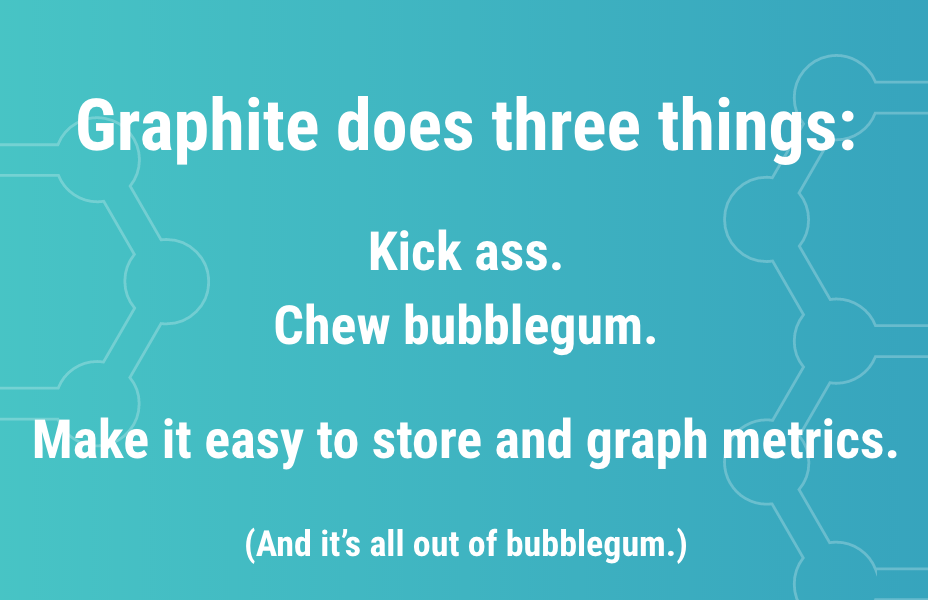
\includegraphics[height=0.4\paperheight]{graphite-official}
		\end{center}
		\caption{From the \href{http://graphiteapp.org}{graphiteapp.org}}
	\end{figure}
	\Large{
	\begin{itemize}
		\item Allows to store time-series data % TODO: check spelling
		\item Easy to use --- text protocol and HTTP API
		\item You can create any data flow you want
		\item Modular --- you can replace any part of it
	\end{itemize}
	}
\end{frame}


\section{Graphite@Booking.com}
\begin{frame}
	\frametitle{Open Source stack}
\begin{figure}[h]
\begin{center}
	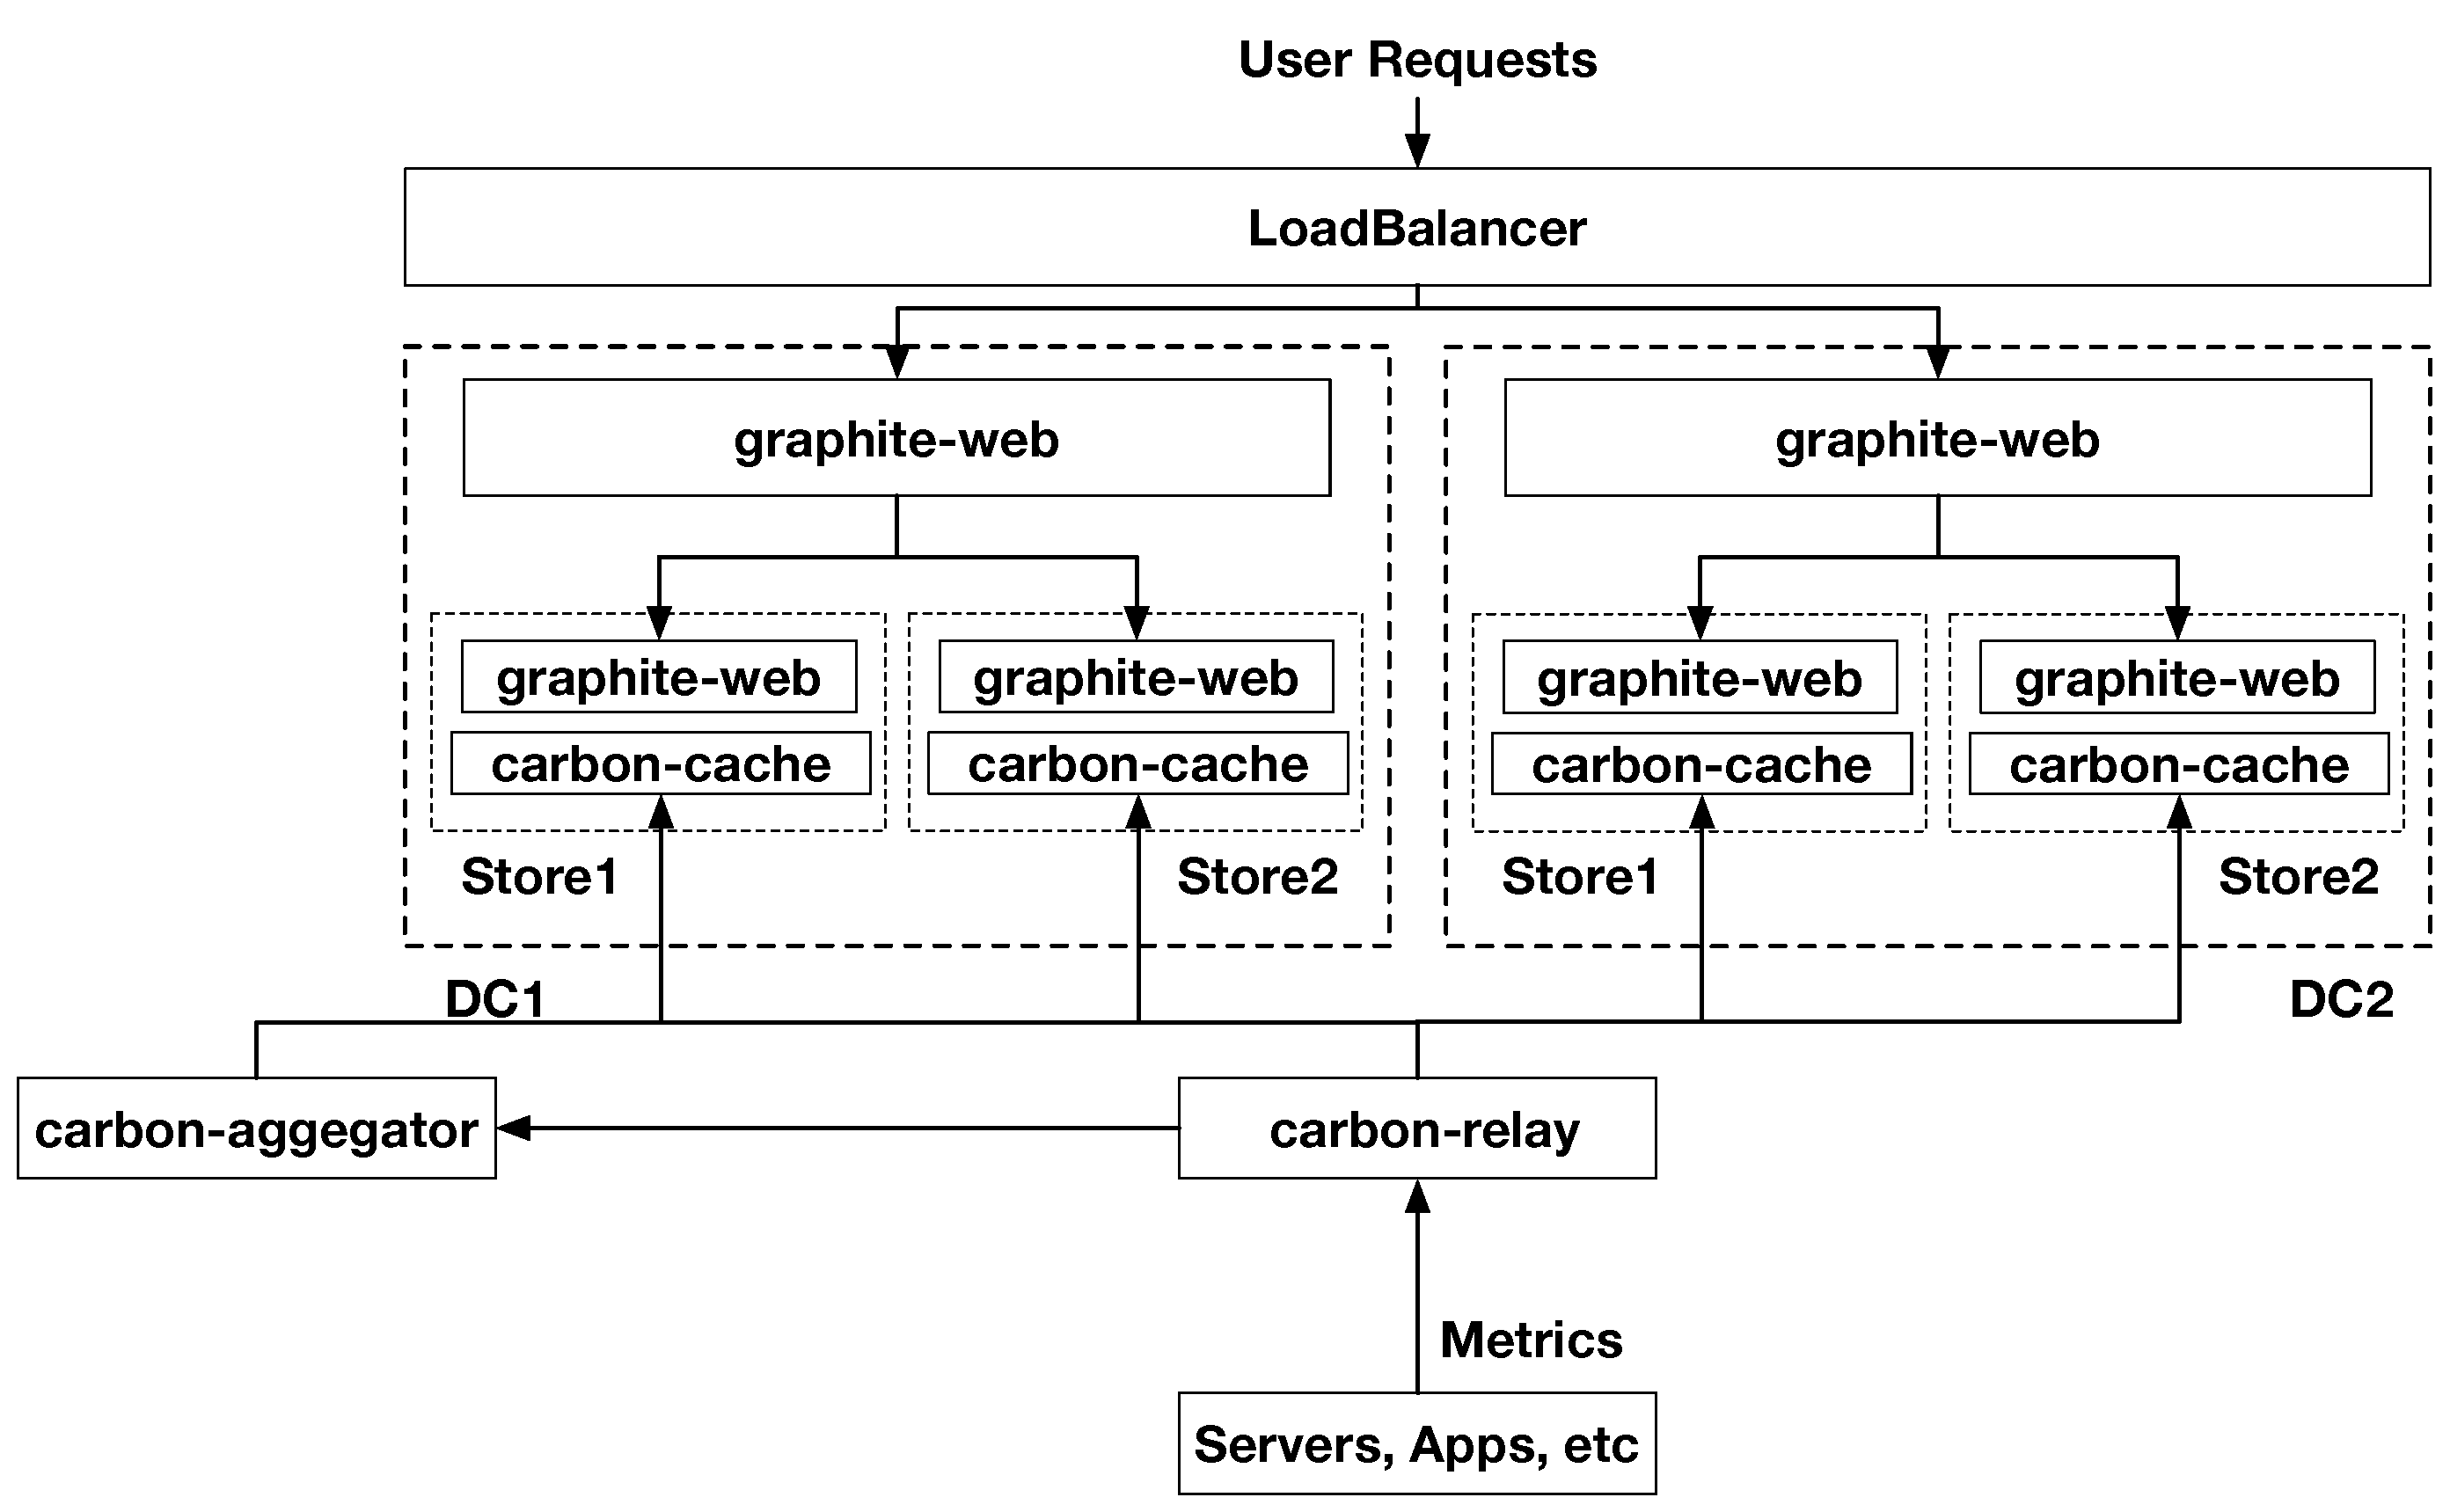
\includegraphics[width=1.05\columnwidth]{graphite-oss}
\end{center}
\end{figure}
\end{frame}

\begin{frame}
	\frametitle{Breaking graphite: our problems at scale}
	\begin{columns}
		\begin{column}{0.5\linewidth}
			\begin{figure}[h]
				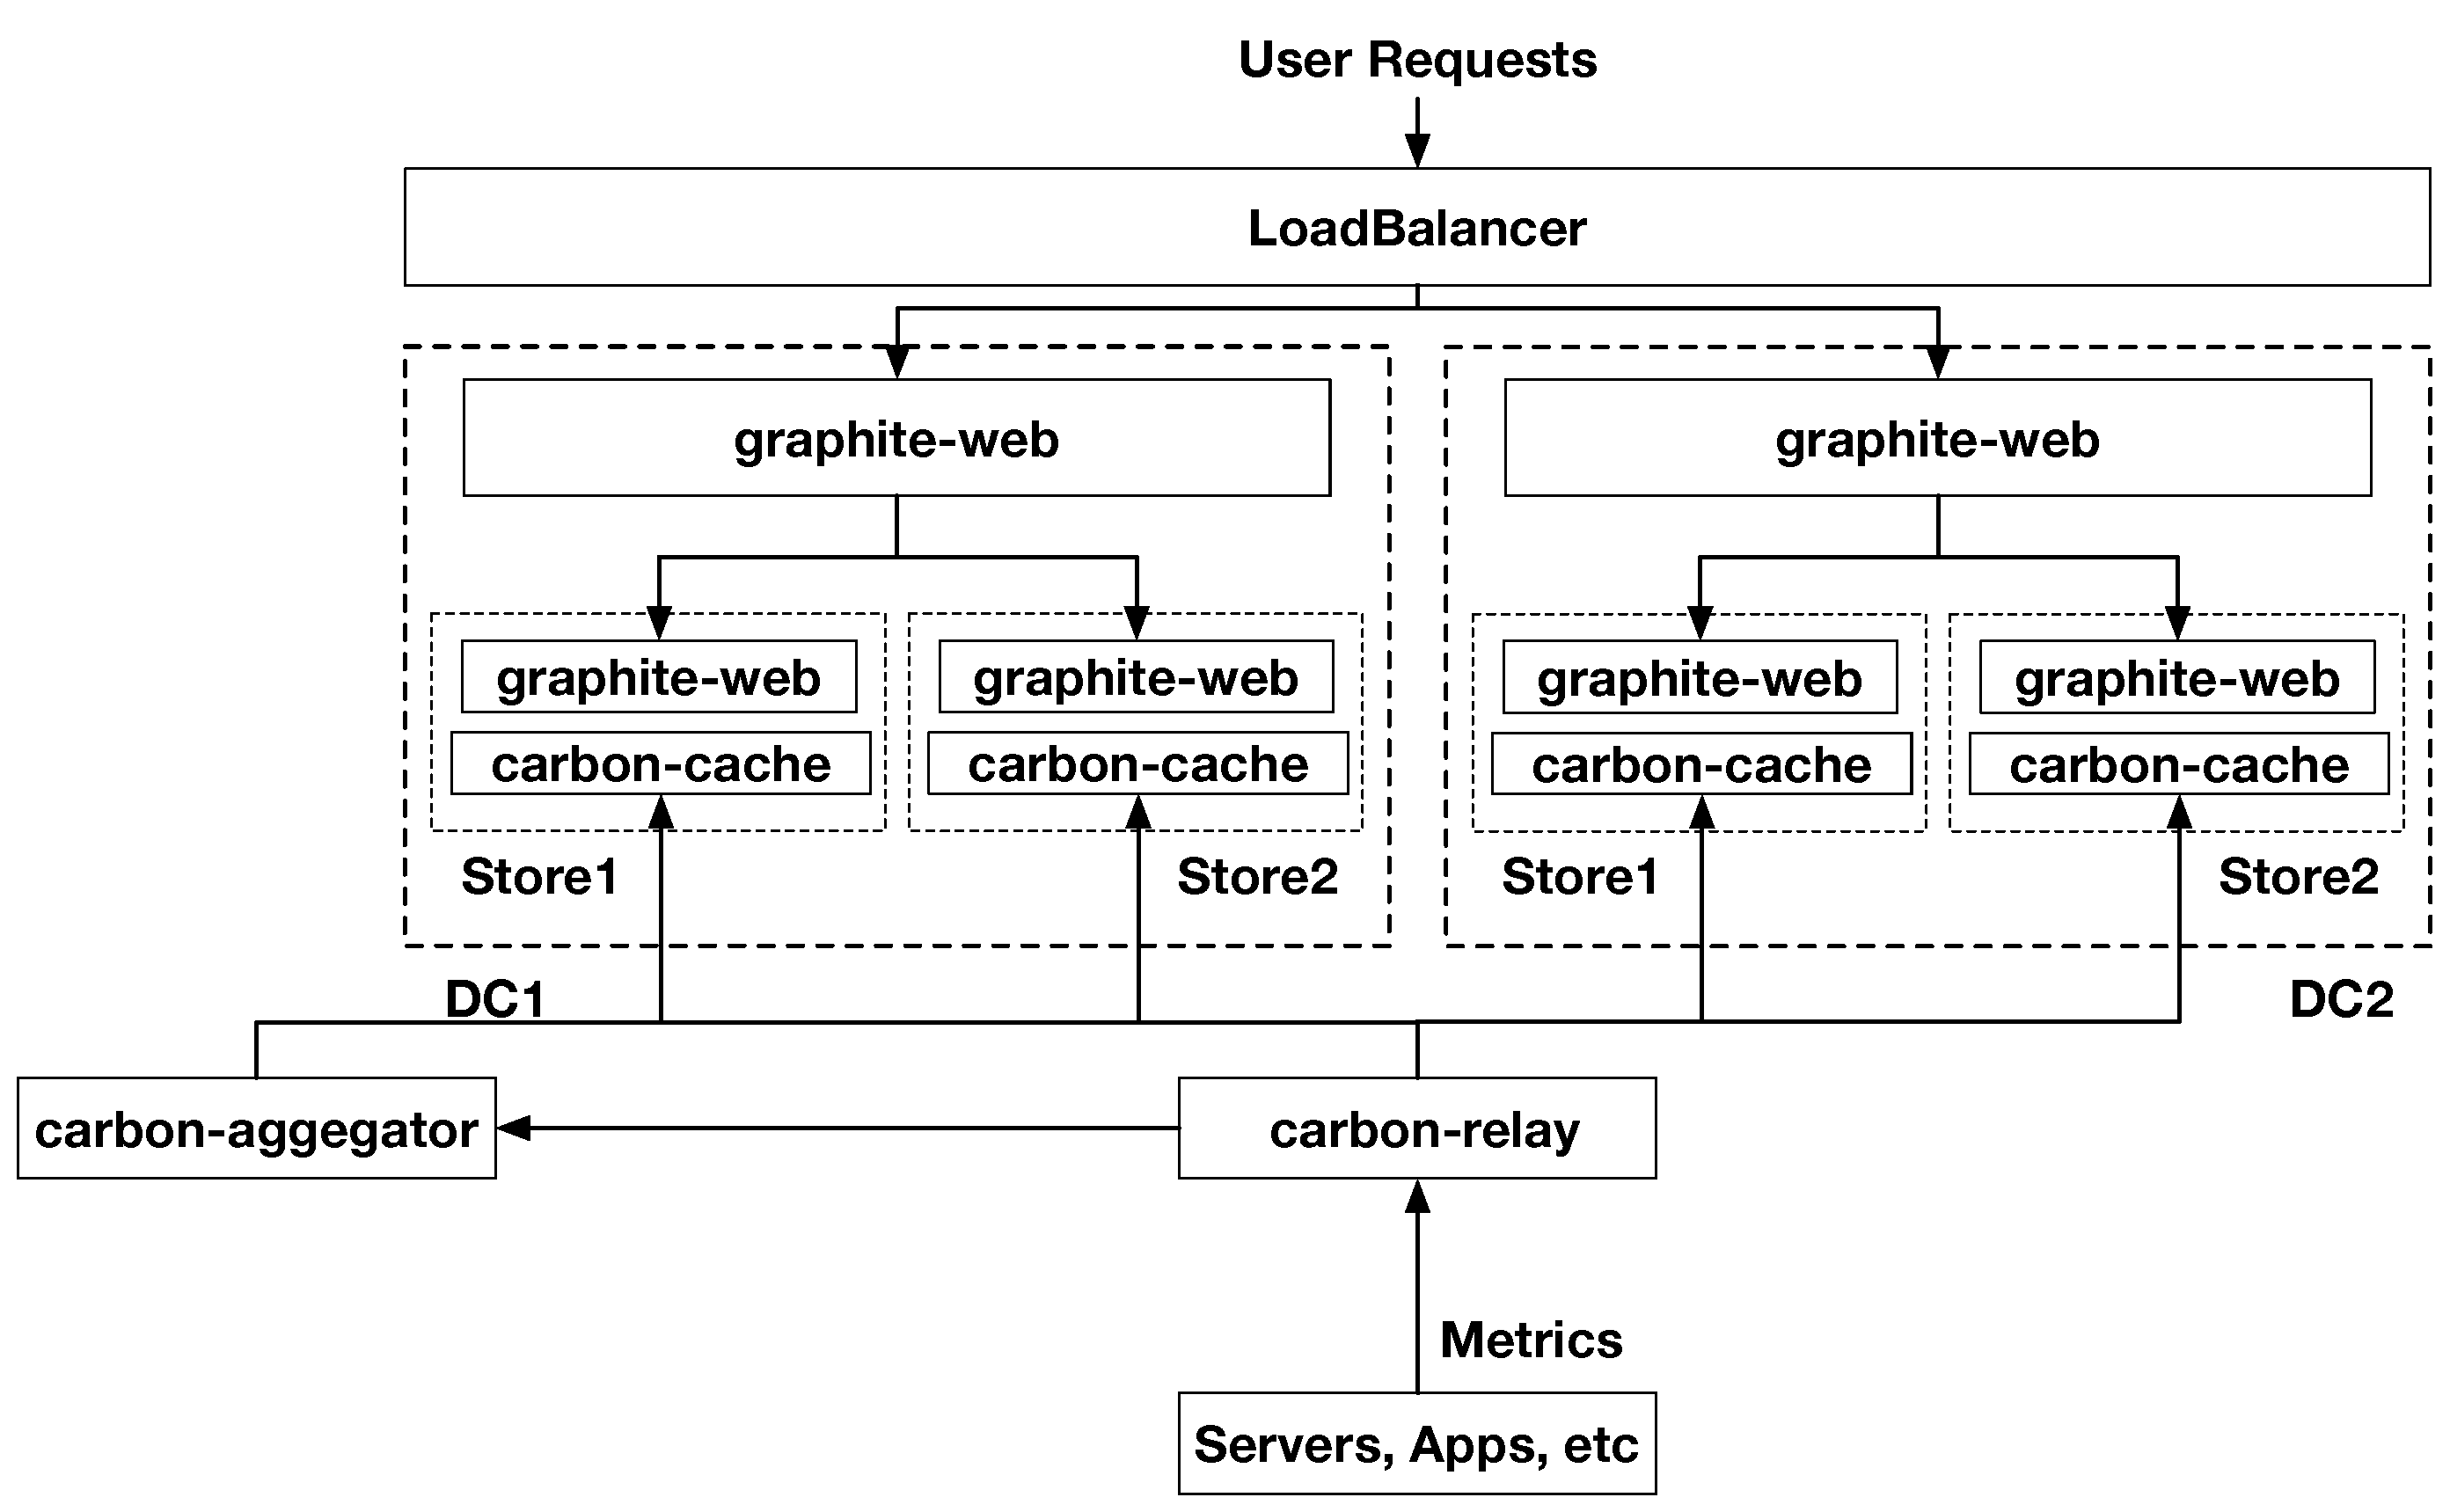
\includegraphics[width=1.0\columnwidth]{graphite-oss}
			\end{figure}
		\end{column}
		\begin{column}{0.5\linewidth}
			\Large{
			What's wrong with this~schema?
			\begin{itemize}
				\item carbon-relay --- SPOF
				\item Hard to scale
				\item Data is different after failures
				\item Render time increases with more servers
			\end{itemize}
			}
		\end{column}
	\end{columns}
\end{frame}

\subsection{Scaling graphite}
\begin{frame}
	\frametitle{Replacing carbon-relay}
	\begin{figure}[h]
		\begin{center}
			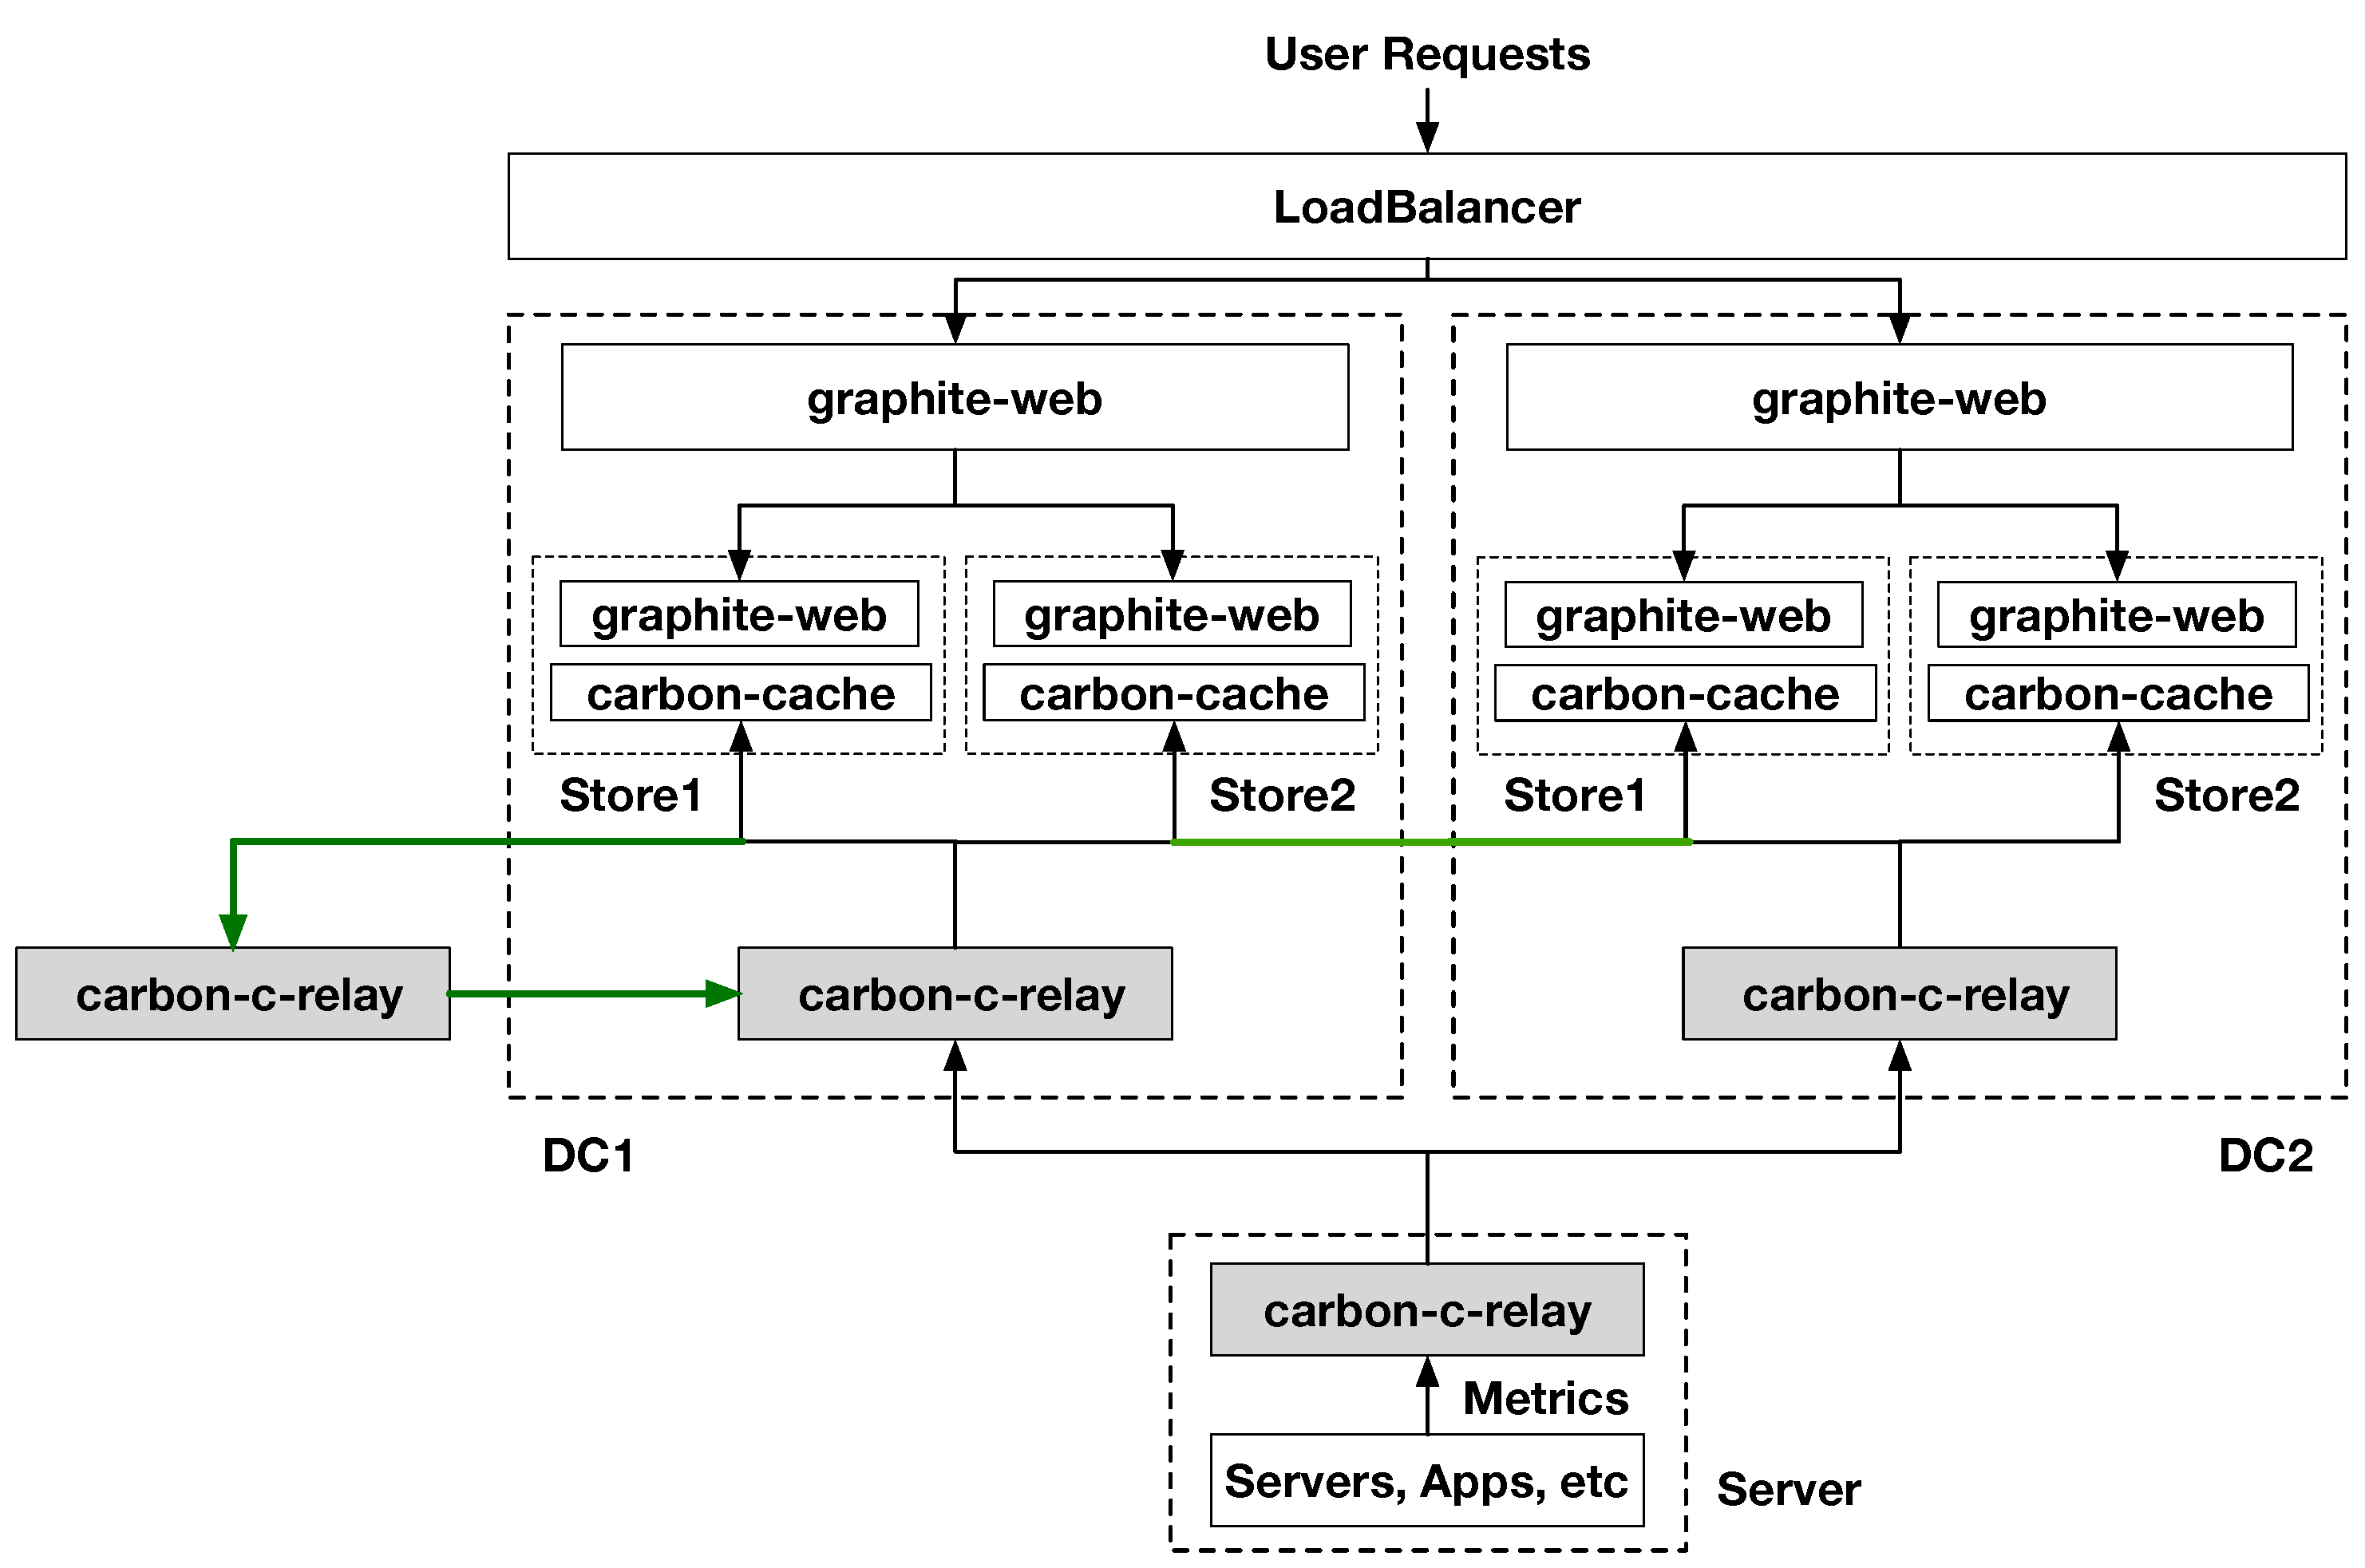
\includegraphics[width=1.05\columnwidth]{graphite-c-relay}
		\end{center}
	\end{figure}
\end{frame}
\begin{frame}
	\frametitle{Replacing carbon-relay}
	\Large{
	carbon-c-relay:
	\begin{itemize}
		\item Written in \bs{C}
		\item Routes \bs{1M} data points per~second using only \bs{2} cores
		\item L7 LB for graphite line protocol (RR with sticking)
		\item Can do aggregations
		\item Buffers the data if upstream is unavailable
	\end{itemize}
	}
\end{frame}

\begin{frame}
	\frametitle{Zipper stack: Solution}
	\Large{
	Query: target=sys.server.cpu.user
	\newline

	Result:
	\newline\newline
	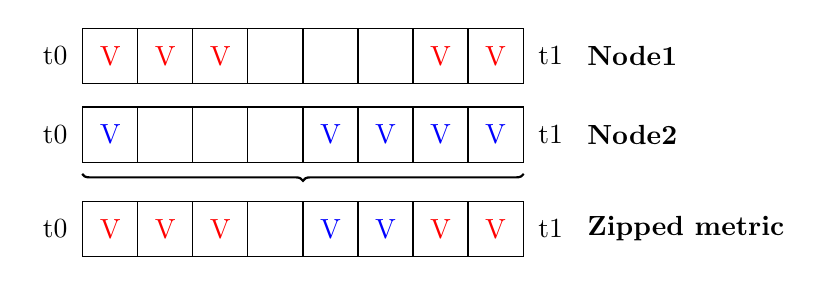
\begin{tikzpicture}
	tikzstyle{every path}=[very thick]

\edef\sizetape{0.7cm}
\tikzstyle{tmtape}=[draw,minimum size=\sizetape]
\tikzstyle{tmhead}=[arrow box,draw,minimum size=.5cm,arrow box
arrows={east:.25cm, west:0.25cm}]

%% Draw TM tape
\begin{scope}[start chain=1 going right,node distance=-0.15mm]
    \node [on chain=1,tmtape,draw=none] {t0};
    \node [on chain=1,tmtape] {\textcolor{red}{V}};
    \node [on chain=1,tmtape] {\textcolor{red}{V}};
    \node [on chain=1,tmtape] {\textcolor{red}{V}};
    \node [on chain=1,tmtape] {};
    \node [on chain=1,tmtape] {};
    \node [on chain=1,tmtape] {};
    \node [on chain=1,tmtape] {\textcolor{red}{V}};
    \node [on chain=1,tmtape] {\textcolor{red}{V}};
    \node [on chain=1,tmtape,draw=none] {t1};
    \node [on chain=1] {\textbf{Node1}};
\end{scope}
\begin{scope}[shift={(0,-1cm)},start chain=1 going right,node distance=-0.15mm]
    \node [on chain=1,tmtape,draw=none] {t0};
    \node (v0)[on chain=1,tmtape] {\textcolor{blue}{V}};
    \node [on chain=1,tmtape] {};
    \node [on chain=1,tmtape] {};
    \node [on chain=1,tmtape] {};
    \node [on chain=1,tmtape] {\textcolor{blue}{V}};
    \node [on chain=1,tmtape] {\textcolor{blue}{V}};
    \node [on chain=1,tmtape] {\textcolor{blue}{V}};
    \node (vl)[on chain=1,tmtape] {\textcolor{blue}{V}};
    \node [on chain=1,tmtape,draw=none] {t1};
    \node [on chain=1] {\textbf{Node2}};
%\draw [
%    snake=coil,
%    segment amplitude=10pt,
%    segment length=5pt
%] (v0.west) -- (vl.east); 
\draw [
    thick,
    decoration={
        brace,
        mirror,
        raise=0.5cm
    },
    decorate
] (v0.west) -- (vl.east);
\end{scope}
\begin{scope}[shift={(0,-2.2cm)},start chain=1 going right,node distance=-0.15mm]
    \node [on chain=1,tmtape,draw=none] {t0};
    \node [on chain=1,tmtape] {\textcolor{red}{V}};
    \node [on chain=1,tmtape] {\textcolor{red}{V}};
    \node [on chain=1,tmtape] {\textcolor{red}{V}};
    \node [on chain=1,tmtape] {};
    \node [on chain=1,tmtape] {\textcolor{blue}{V}};
    \node [on chain=1,tmtape] {\textcolor{blue}{V}};
    \node [on chain=1,tmtape] {\textcolor{red}{V}};
    \node [on chain=1,tmtape] {\textcolor{red}{V}};
    \node [on chain=1,tmtape,draw=none] {t1};
    \node [on chain=1] {\textbf{Zipped metric}};
\end{scope}
	\end{tikzpicture}
	}
\end{frame}

%\begin{frame}
%	\frametitle{Zipper stack: architecture recap}
%	\begin{figure}[h]
%		\begin{center}
%			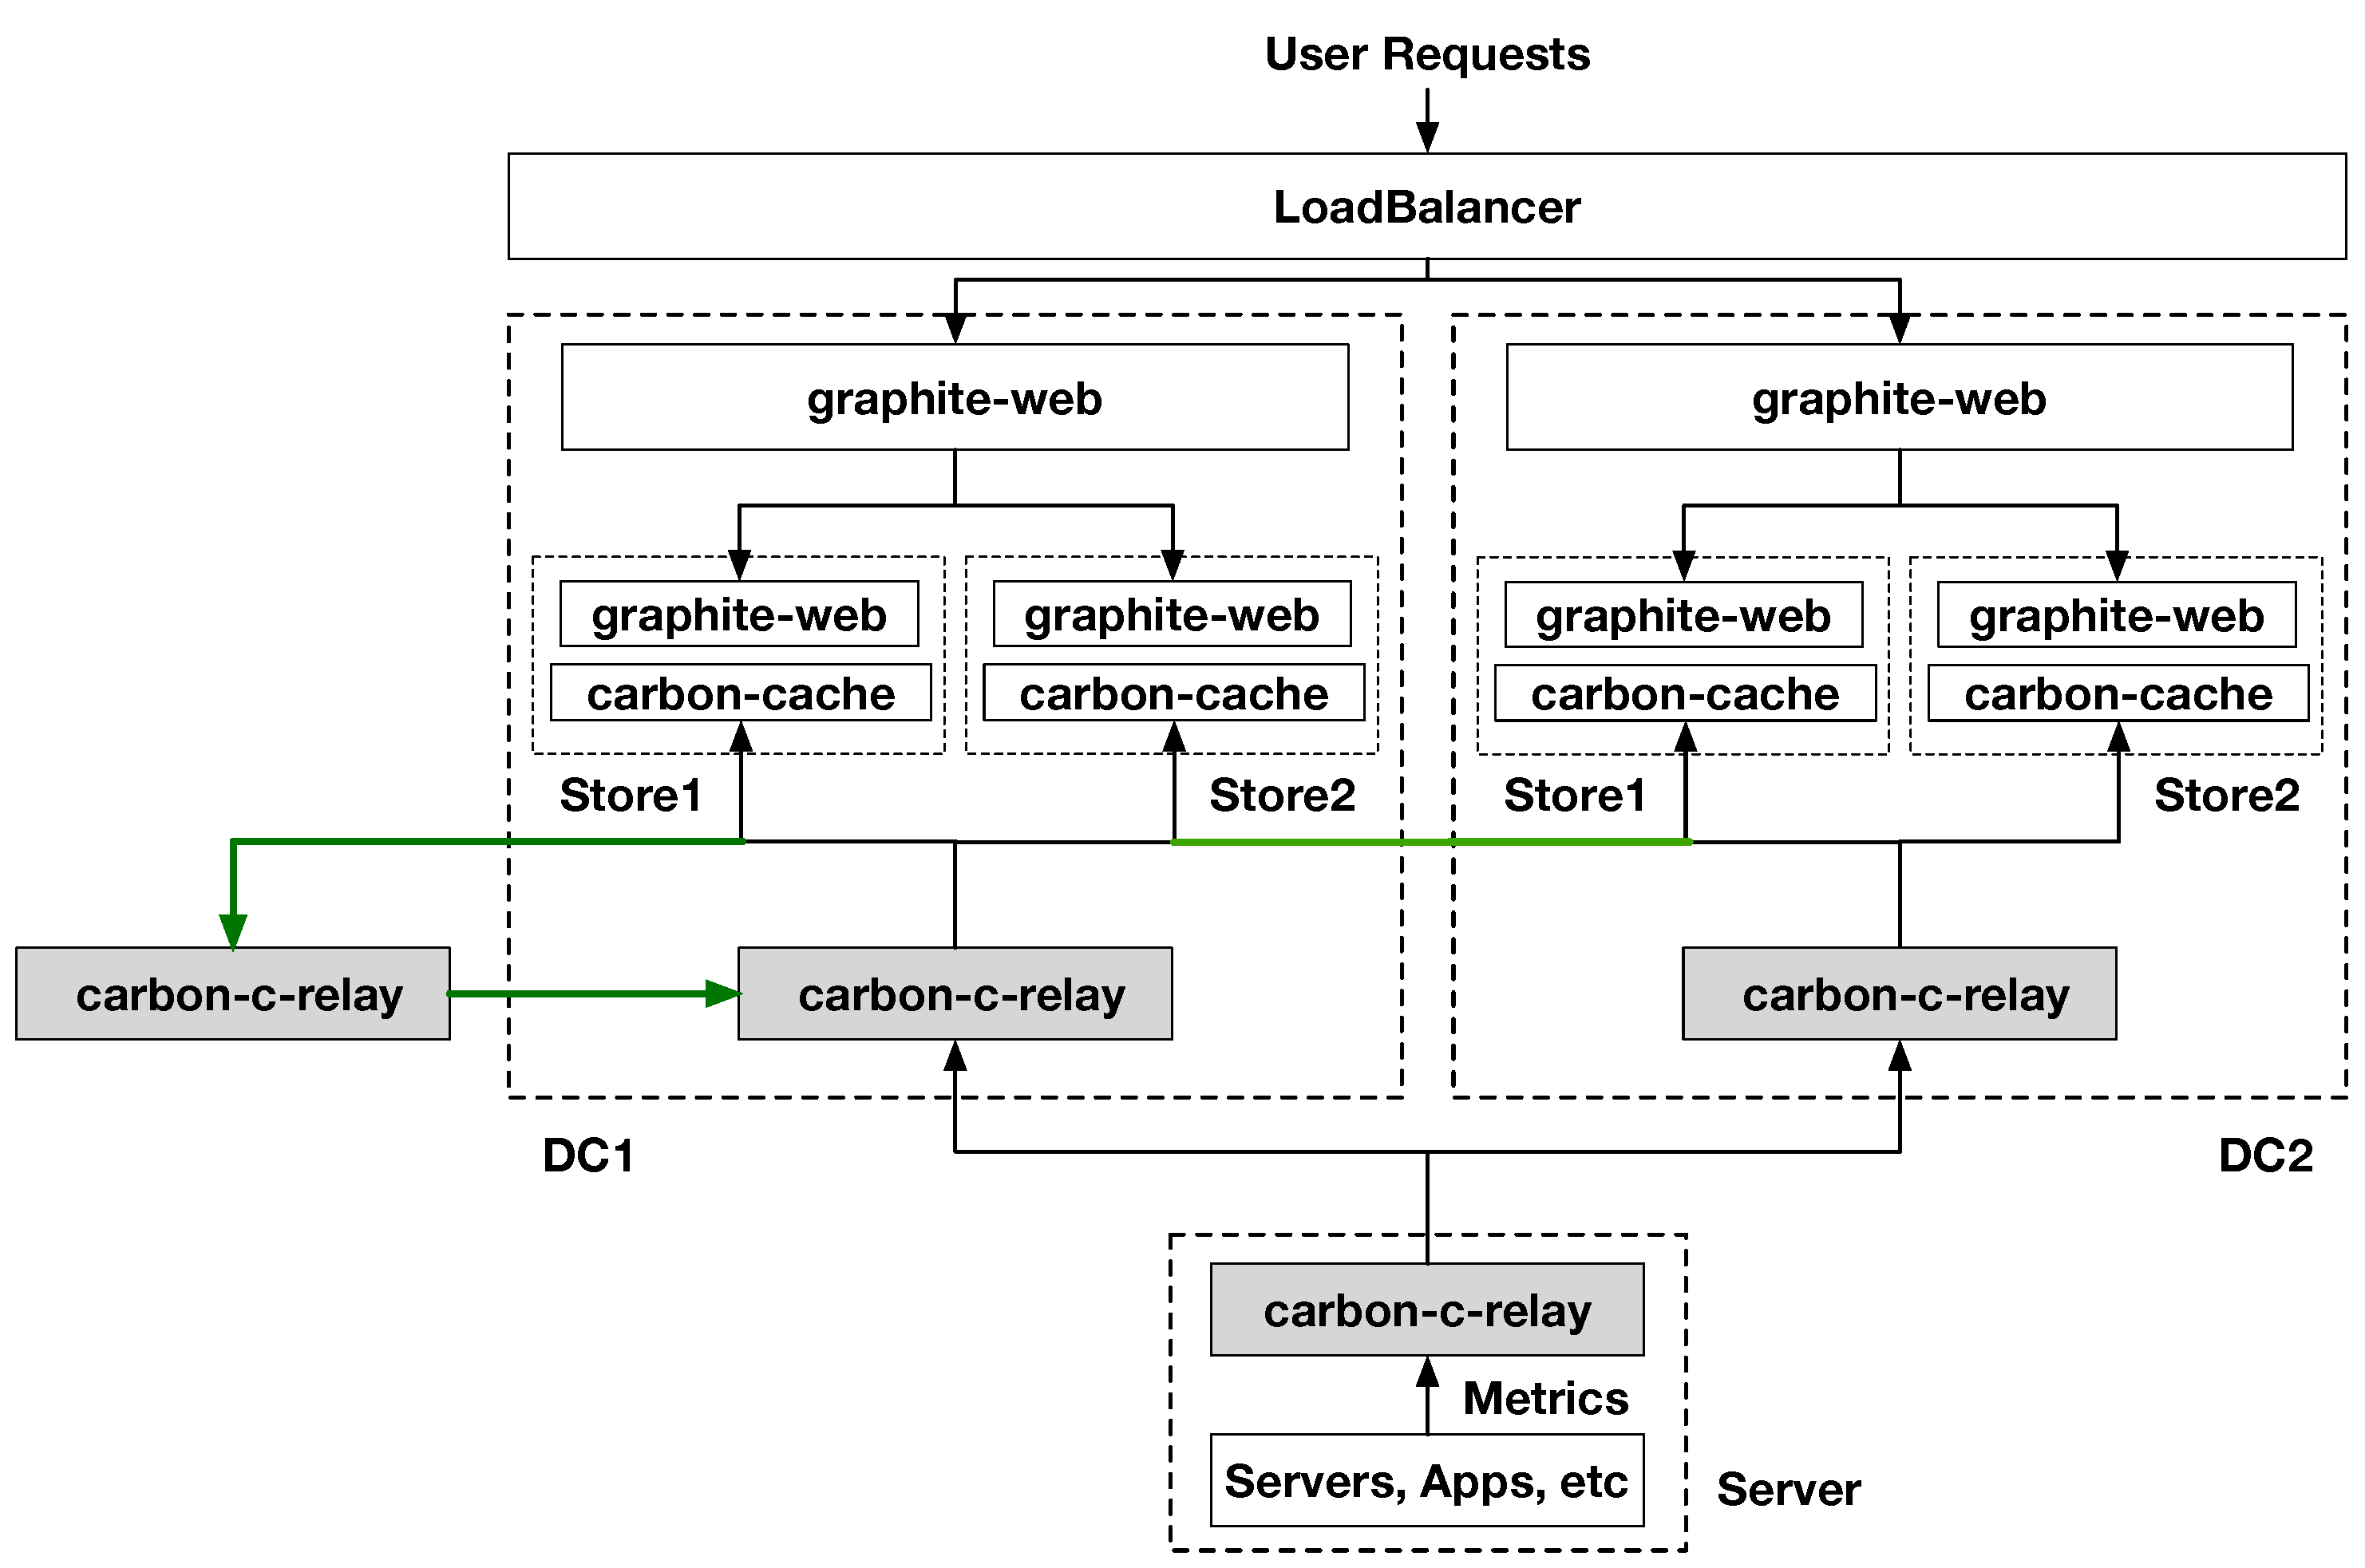
\includegraphics[width=0.7\columnwidth]{graphite-c-relay}
%		\end{center}
%	\end{figure}
%	\transdissolve
%\end{frame}

\begin{frame}
	\frametitle{Zipper stack: architecture}
	\begin{figure}[h]
		\begin{center}
			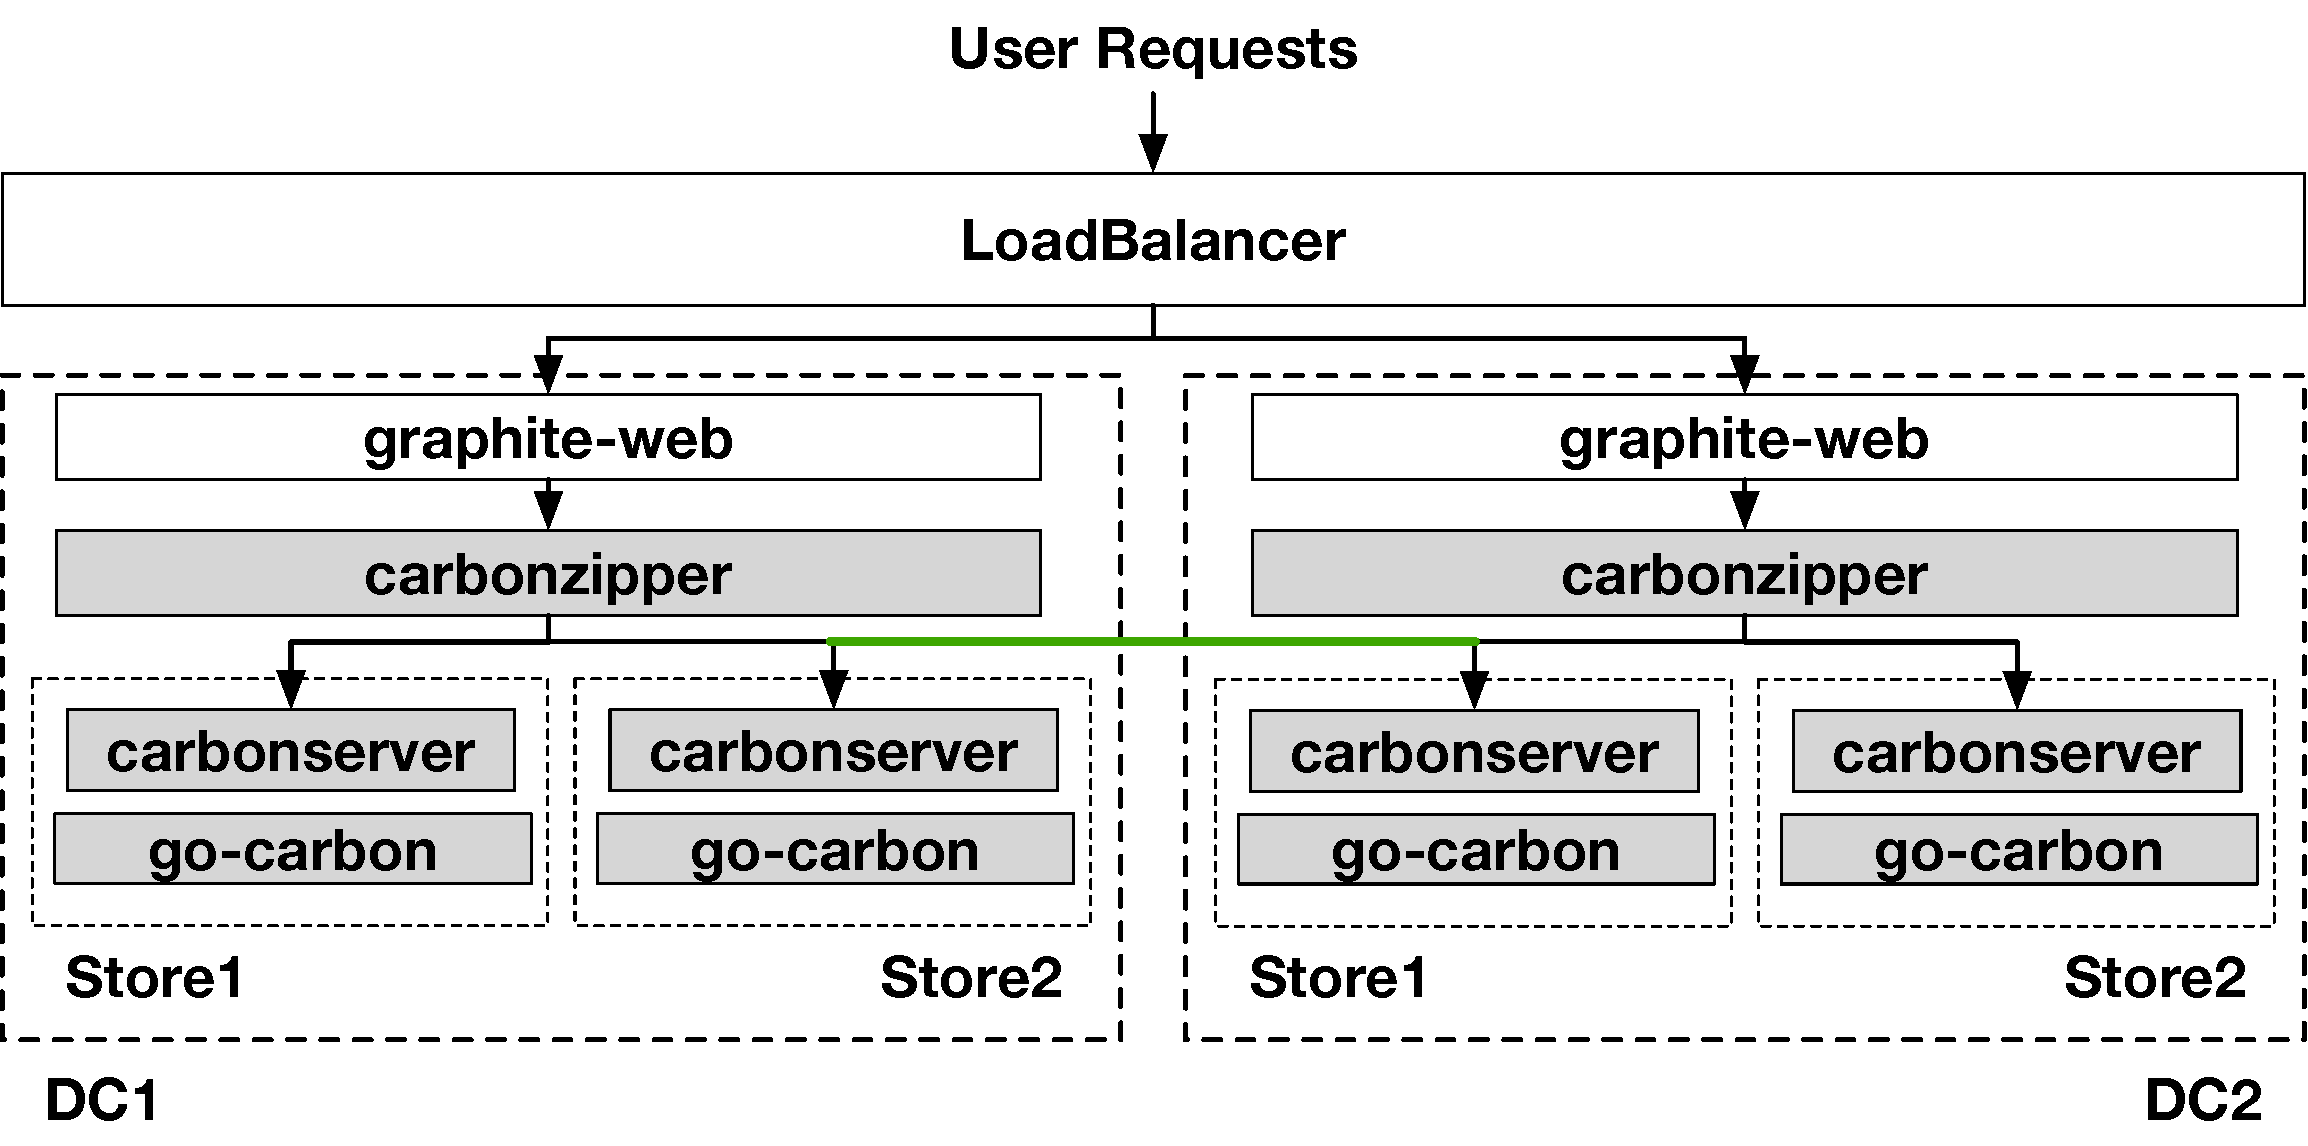
\includegraphics[width=1.05\columnwidth]{graphite-zipper}
		\end{center}
	\end{figure}
\end{frame}

\begin{frame}
	\frametitle{Zipper stack: results}
	\Large{
	\begin{itemize}
	\item Written in \bs{Go}
	\item Can query store servers in \bs{parallel}
	\item Can "Zip" the data
	\item carbonzipper $\Leftrightarrow$ carbonserver --- \bs{2700} RPS

	graphite-web $\Leftrightarrow$ carbon-cache --- \bs{80} RPS.

	\item carbonserver is now part of go-carbon (since December 2016)

	\end{itemize}
	}
\end{frame}

\begin{frame}
	\frametitle{Metric distribution: how it works}
	\begin{figure}[h]
		\begin{center}
			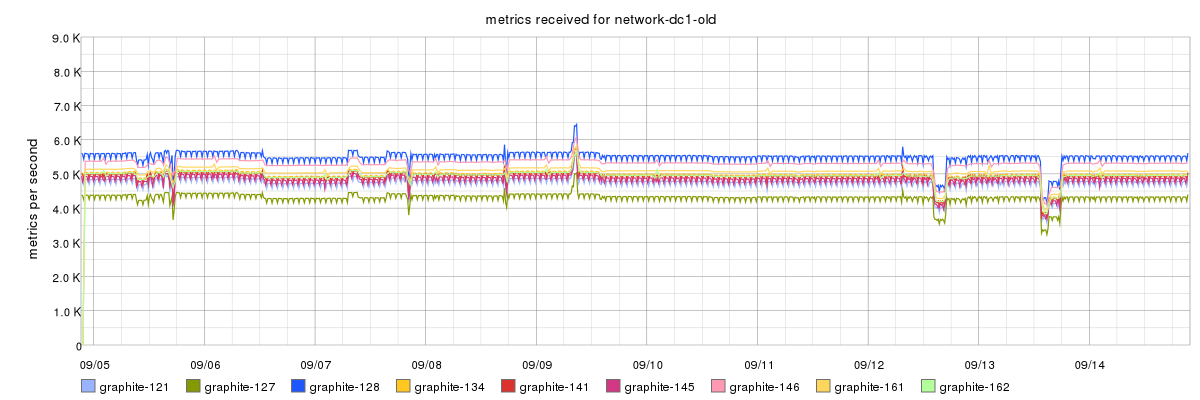
\includegraphics[width=1.05\columnwidth]{graphite-old-hash}
		\end{center}
	\end{figure}
	\Large{
	Up to \bs{20\%} difference in worst case
	}
\end{frame}

\begin{frame}
	\frametitle{Metric distribution: jump hash}
	\begin{figure}[h]
		\begin{center}
			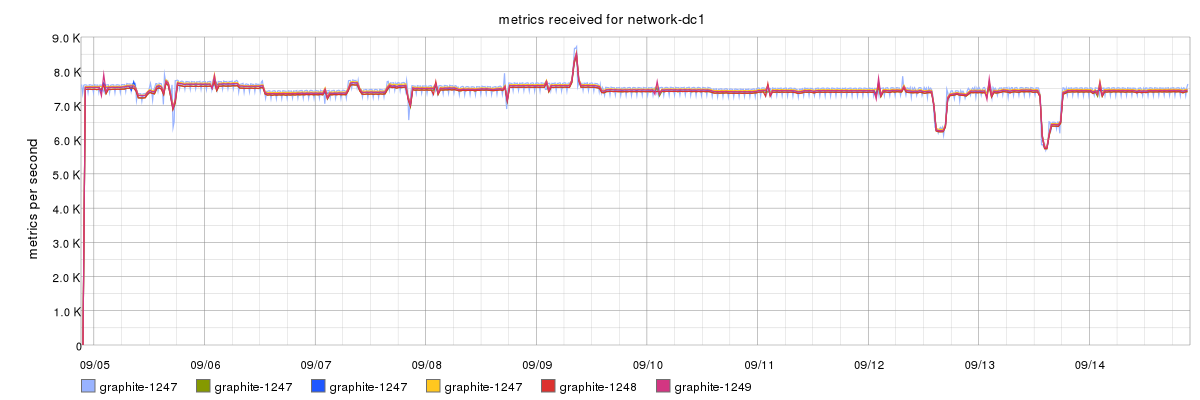
\includegraphics[width=1.05\columnwidth]{graphite-jump-hash}
		\end{center}
	\end{figure}

	\href{https://arxiv.org/pdf/1406.2294v1.pdf}{arxiv.org/pdf/1406.2294v1.pdf}
\end{frame}

\begin{frame}
	\frametitle{Rewriting Frontend in Go: carbonapi}
	\begin{figure}[h]
		\begin{center}
			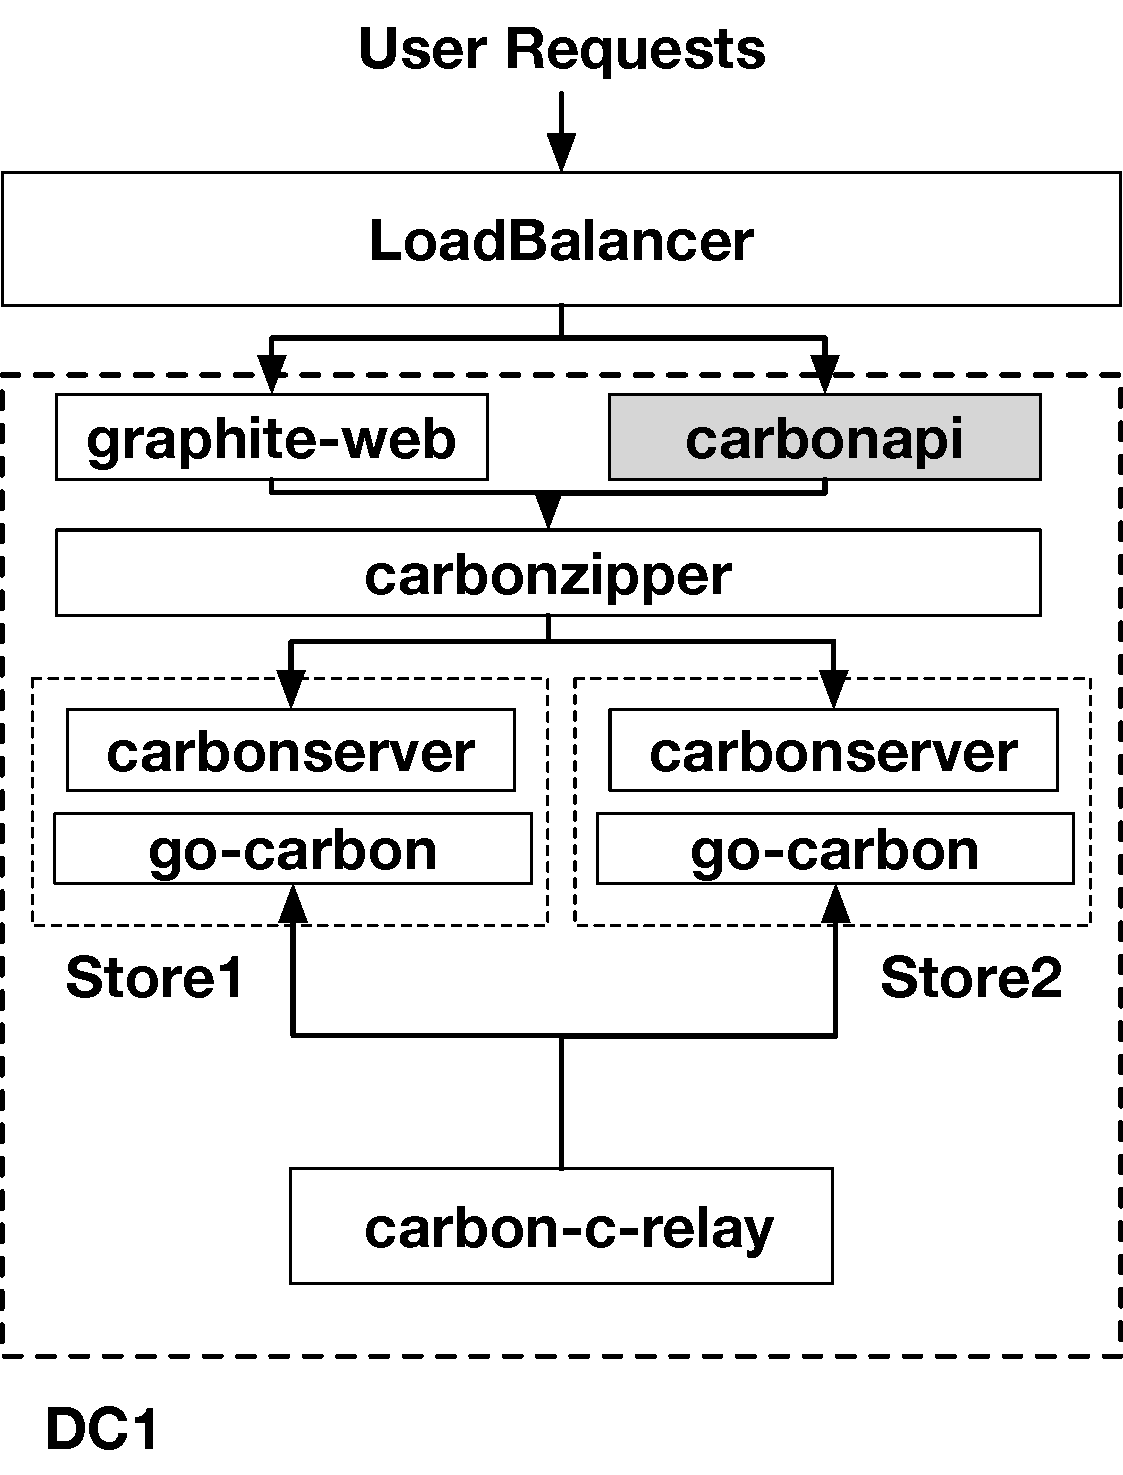
\includegraphics[height=0.8\paperheight]{graphite-carbonapi}
		\end{center}
	\end{figure}
\end{frame}

\begin{frame}
	\frametitle{Rewriting Frontend in Go: result}
	\begin{figure}[h]
		\begin{center}
			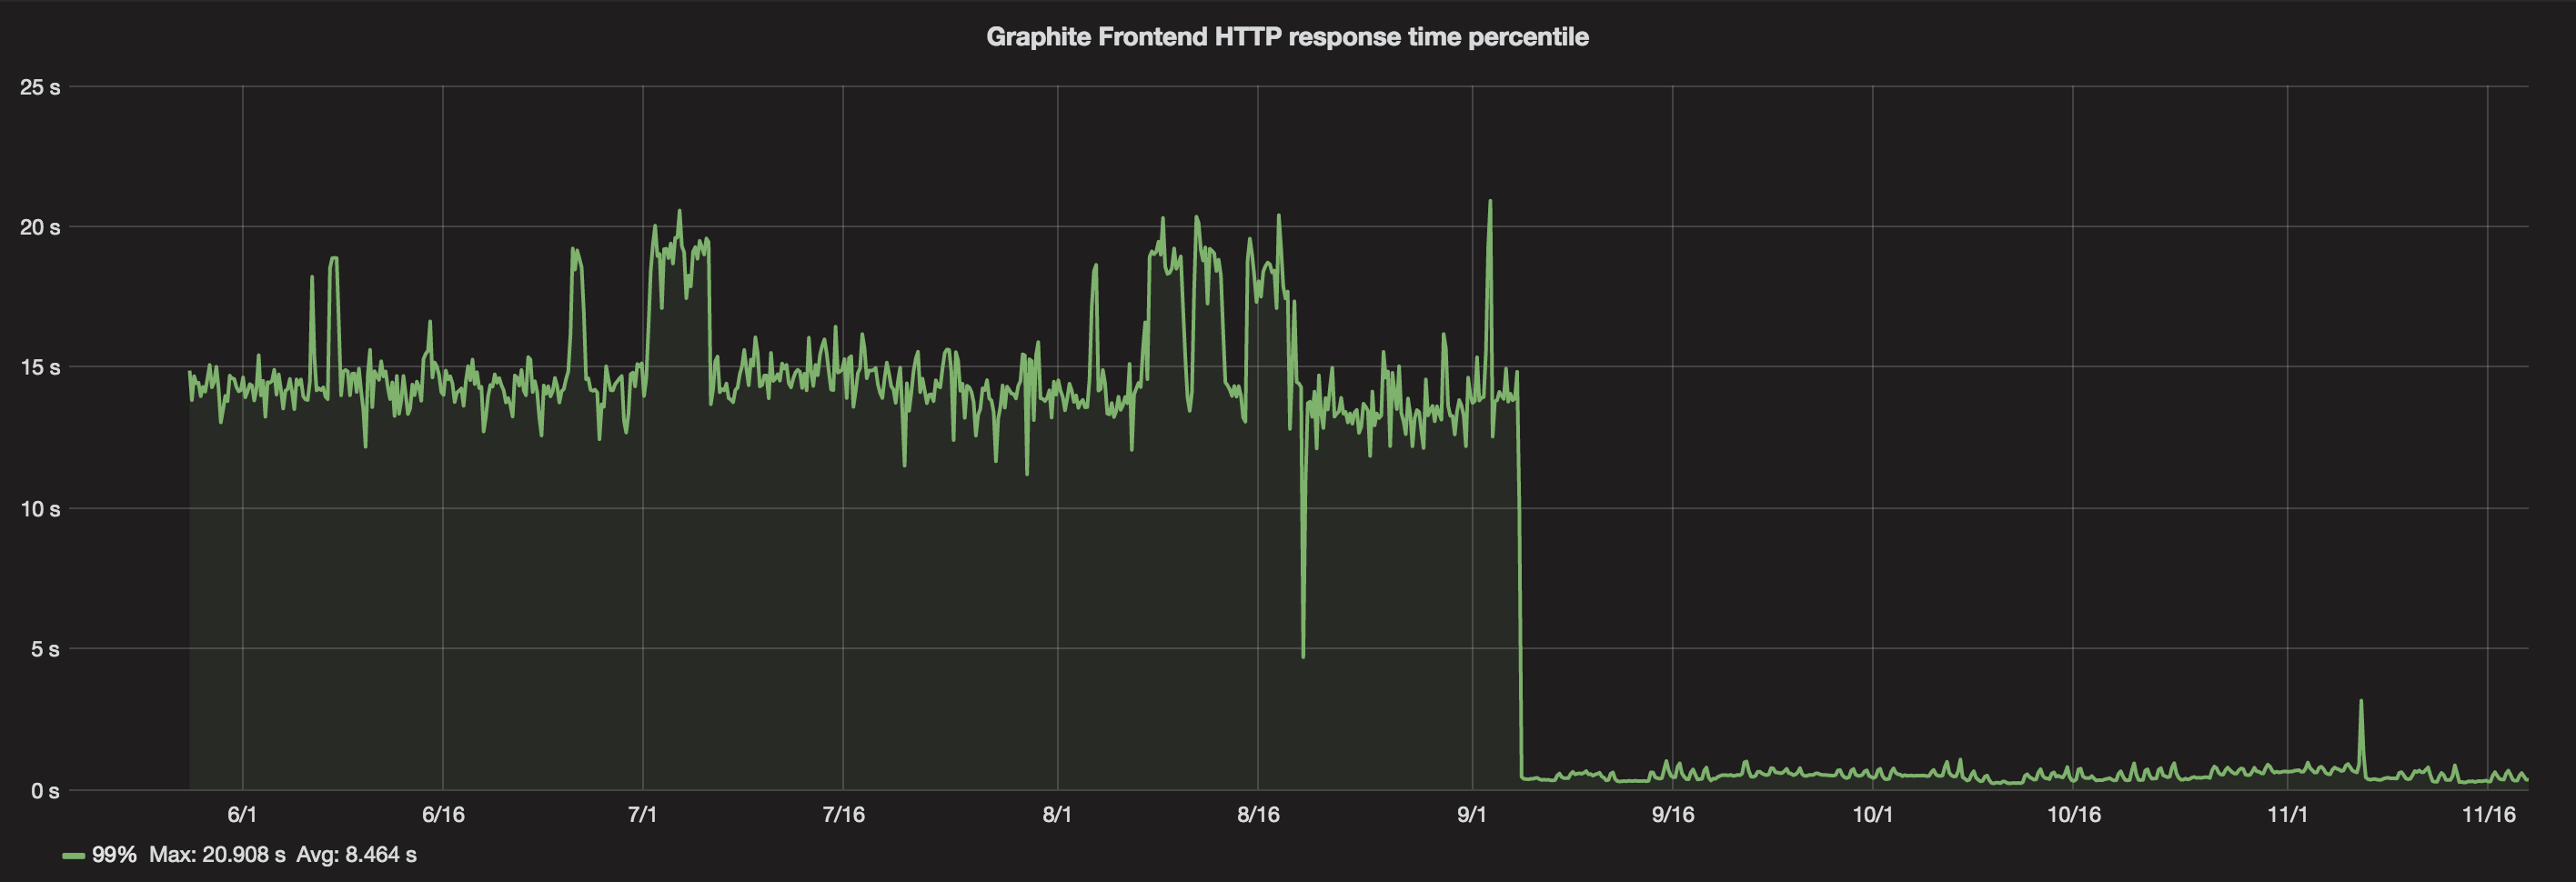
\includegraphics[width=0.9\columnwidth]{graphite-carbonapi-performance}
		\end{center}
	\end{figure}
	\Large{
	\begin{itemize}
		\item Significantly reduced response time for users (\bs{15s $\Rightarrow$ 0.8s})
		\item Allowes more complex queries because it's faster
		\item Easier to implement new heavy math functions
		\item Also available as Go library
	\end{itemize}
	}
\end{frame}


\begin{frame}
%	\frametitle{Metric distribution: the problem}
	\frametitle{Replication techniques and their pros and cons}
%	\begin{columns}
%	\begin{column}{0.5\linewidth}
	\begin{figure}[h]
		\begin{center}
			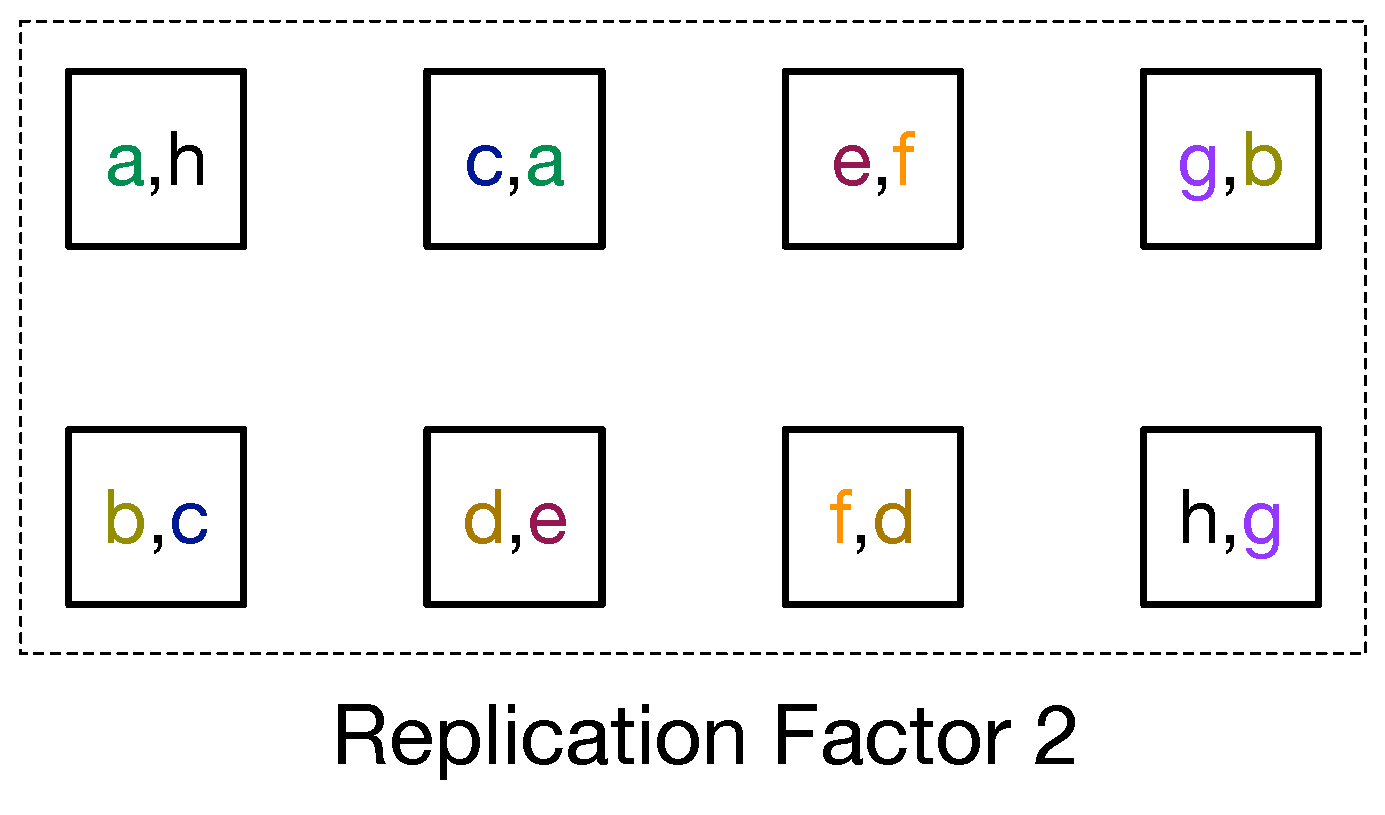
\includegraphics[height=0.7\paperheight]{rf2}
		\end{center}
	\end{figure}
\end{frame}

\begin{frame}
%	\frametitle{Metric distribution: the problem}
	\frametitle{Replication techniques and their pros and cons}
%	\end{column}
%	\begin{column}{0.5\linewidth}
	\begin{figure}[h]
		\begin{center}
			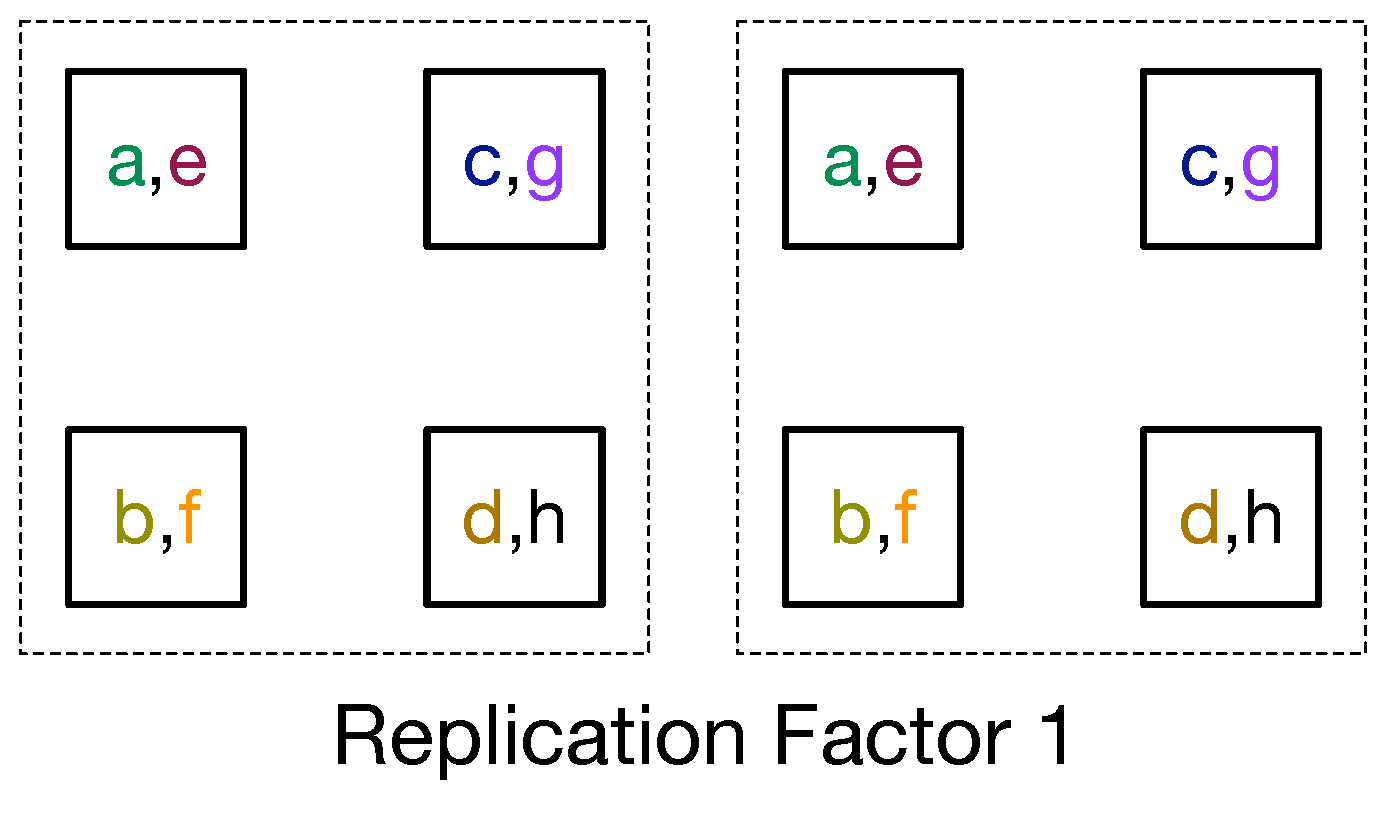
\includegraphics[height=0.7\paperheight]{rf1}
		\end{center}
	\end{figure}
\end{frame}

\begin{frame}
%	\frametitle{Metric distribution: the problem}
	\frametitle{Replication techniques and their pros and cons}
%	\end{column}
%	\end{columns}
	\begin{figure}[h]
		\begin{center}
			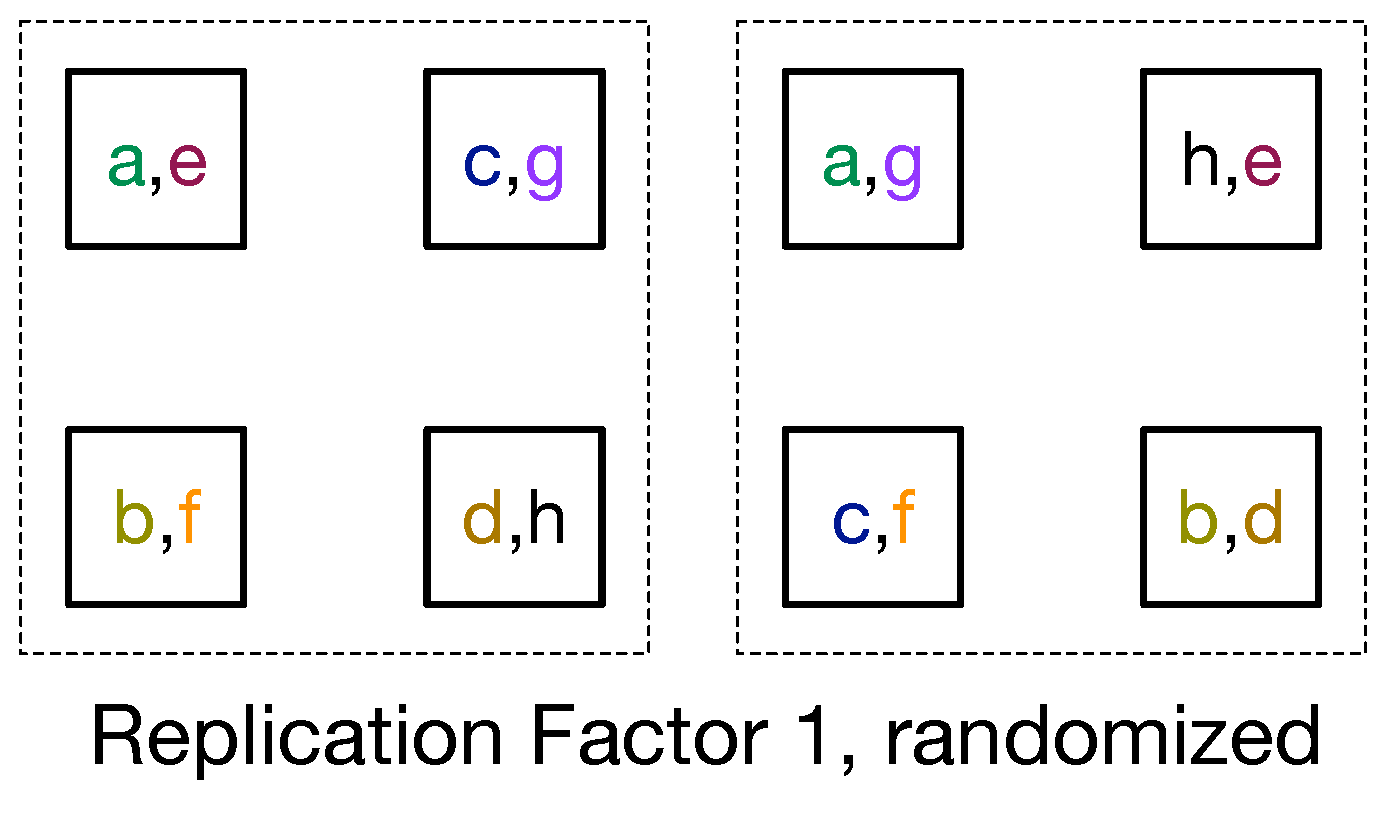
\includegraphics[height=0.7\paperheight]{rf1-rnd}
		\end{center}
	\end{figure}
\end{frame}


\begin{frame}
	\frametitle{Replication techniques and their pros and cons}
	% TODO: fix graph, either remove the title, or make it larger
	\begin{figure}[h]
		\begin{center}
			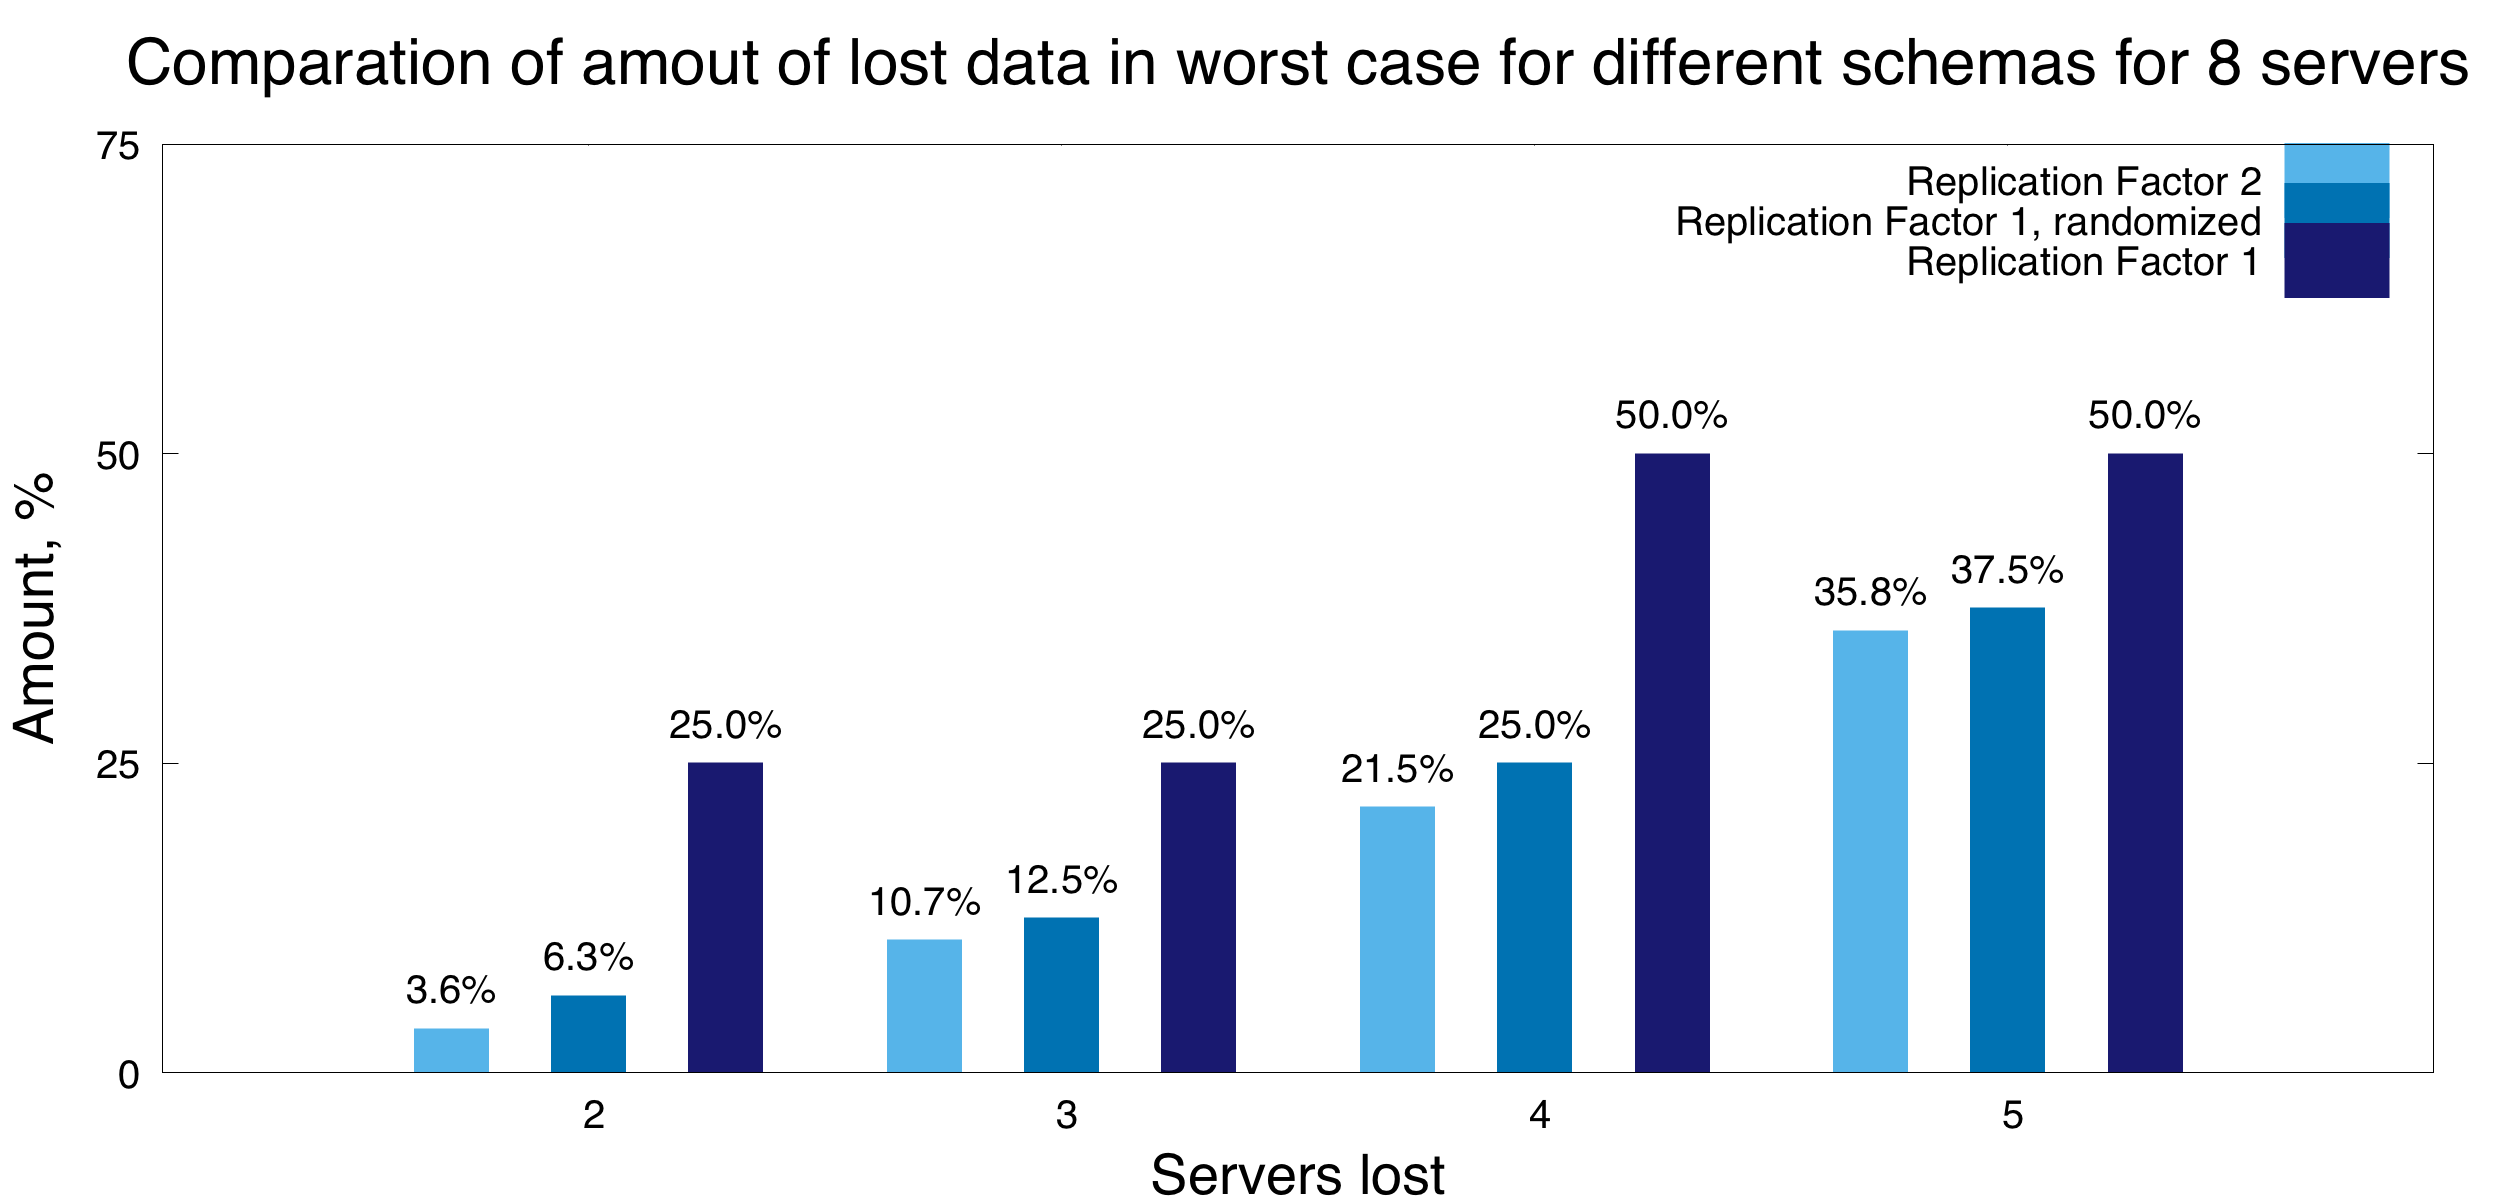
\includegraphics[width=1.05\columnwidth]{experiment_8srv_cmp_al}
		\end{center}
	\end{figure}
\end{frame}
\begin{frame}
	\frametitle{Replication techniques and their pros and cons}
	\begin{figure}[h]
		\begin{center}
			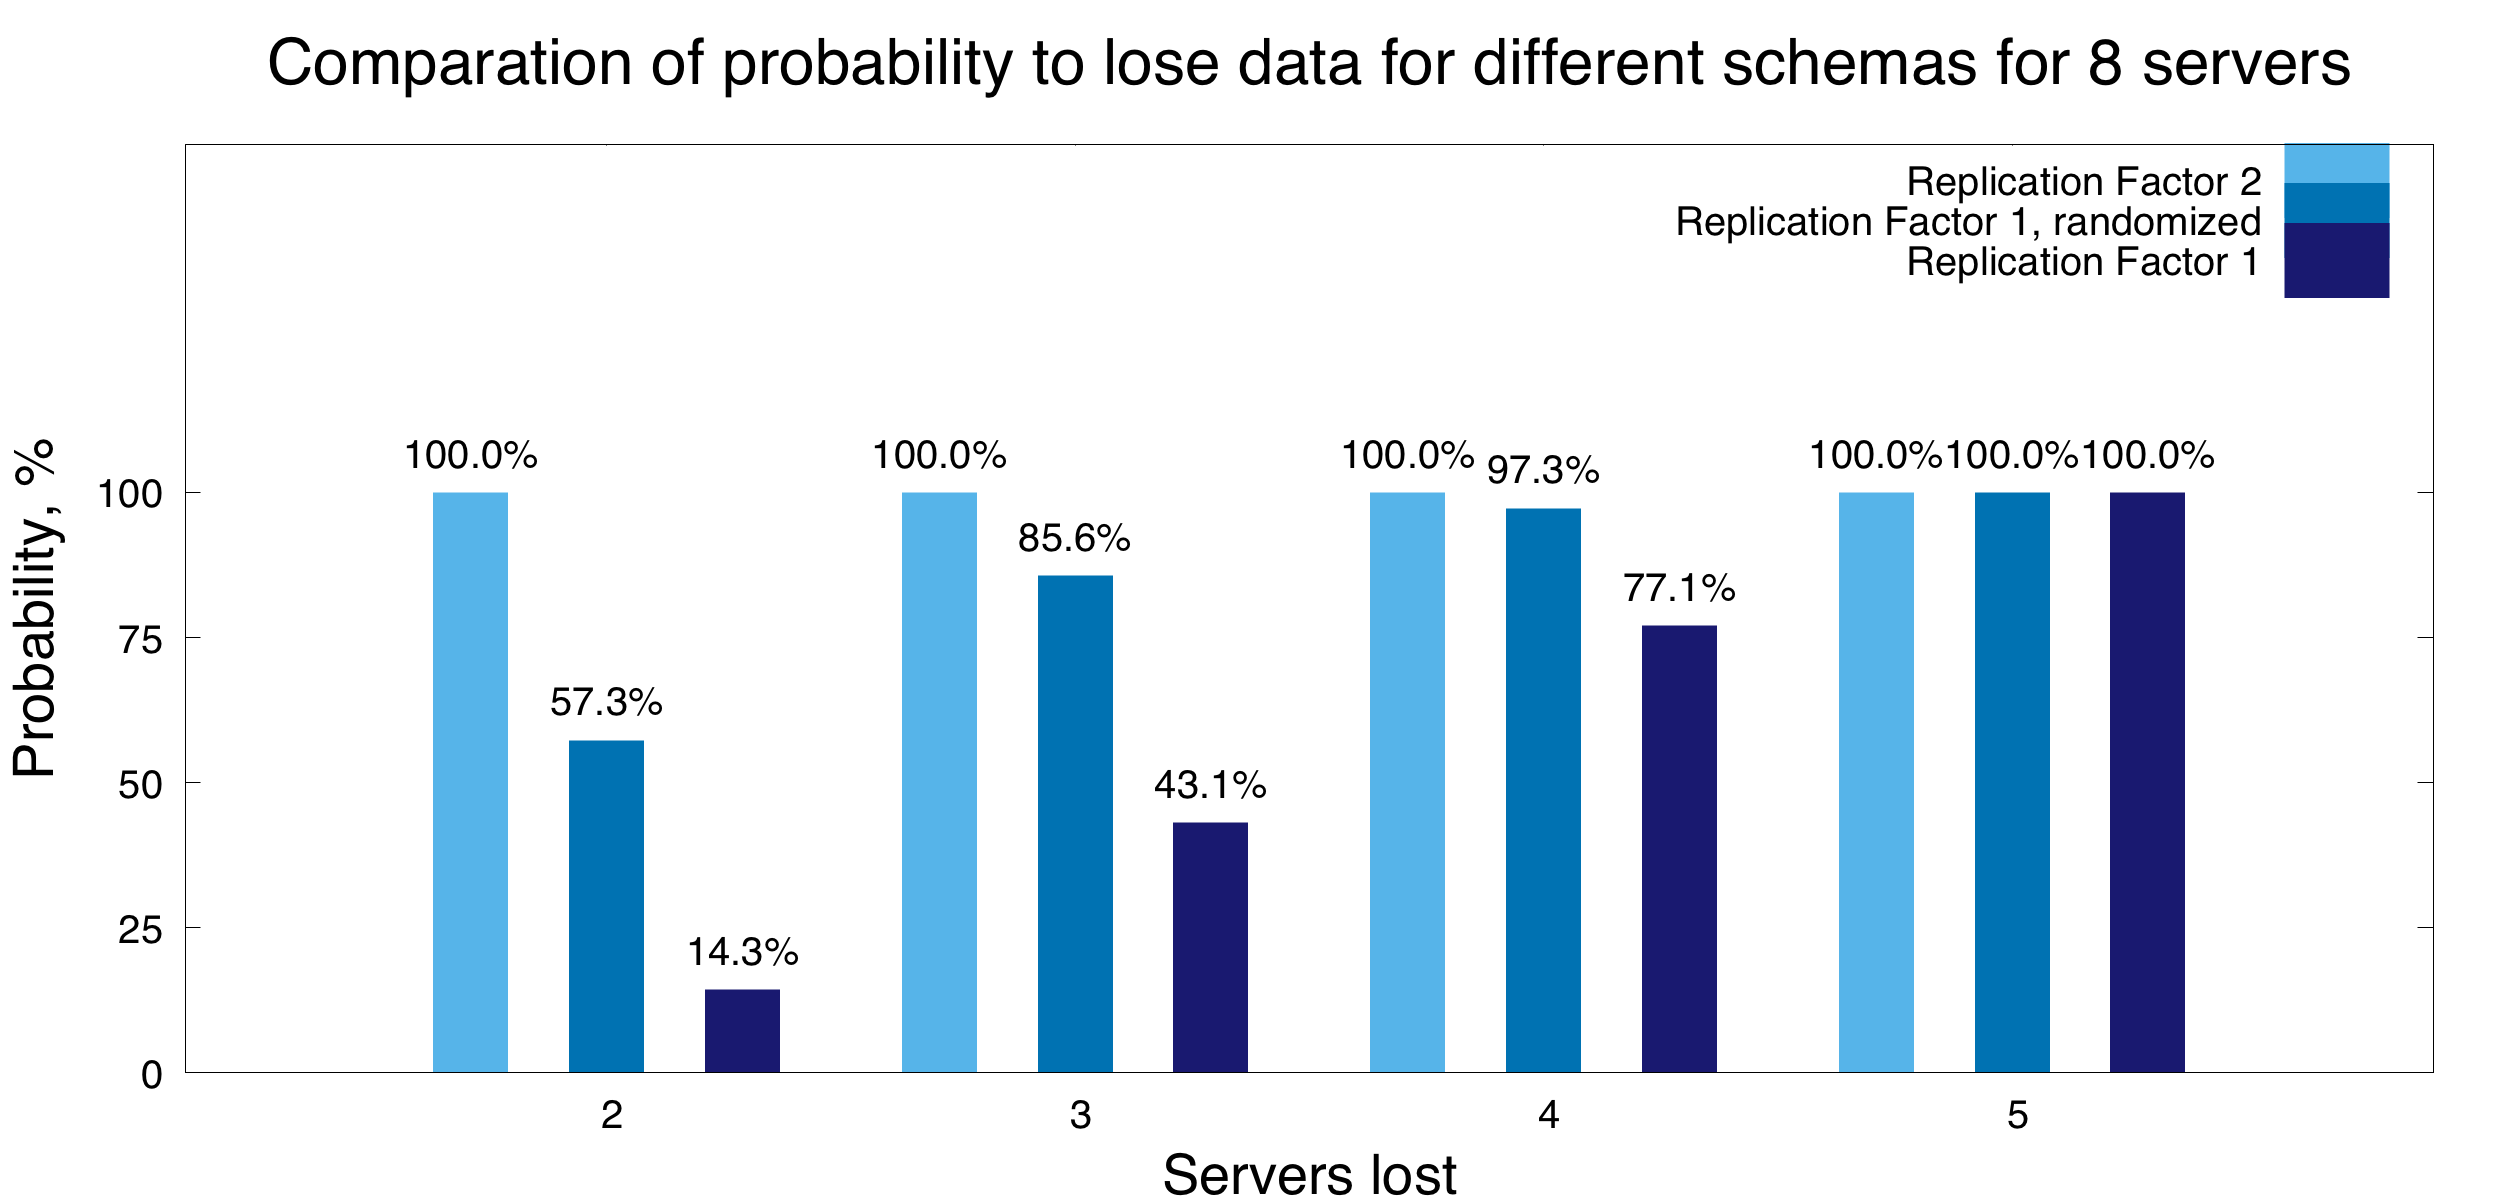
\includegraphics[width=1.05\columnwidth]{experiment_8srv_cmp_cl}
		\end{center}
	\end{figure}

\end{frame}

\section{Summary of technology stack we've built}
\begin{frame}
	\frametitle{Our current setup}
%	\begin{figure}[h]
%		\begin{center}
%			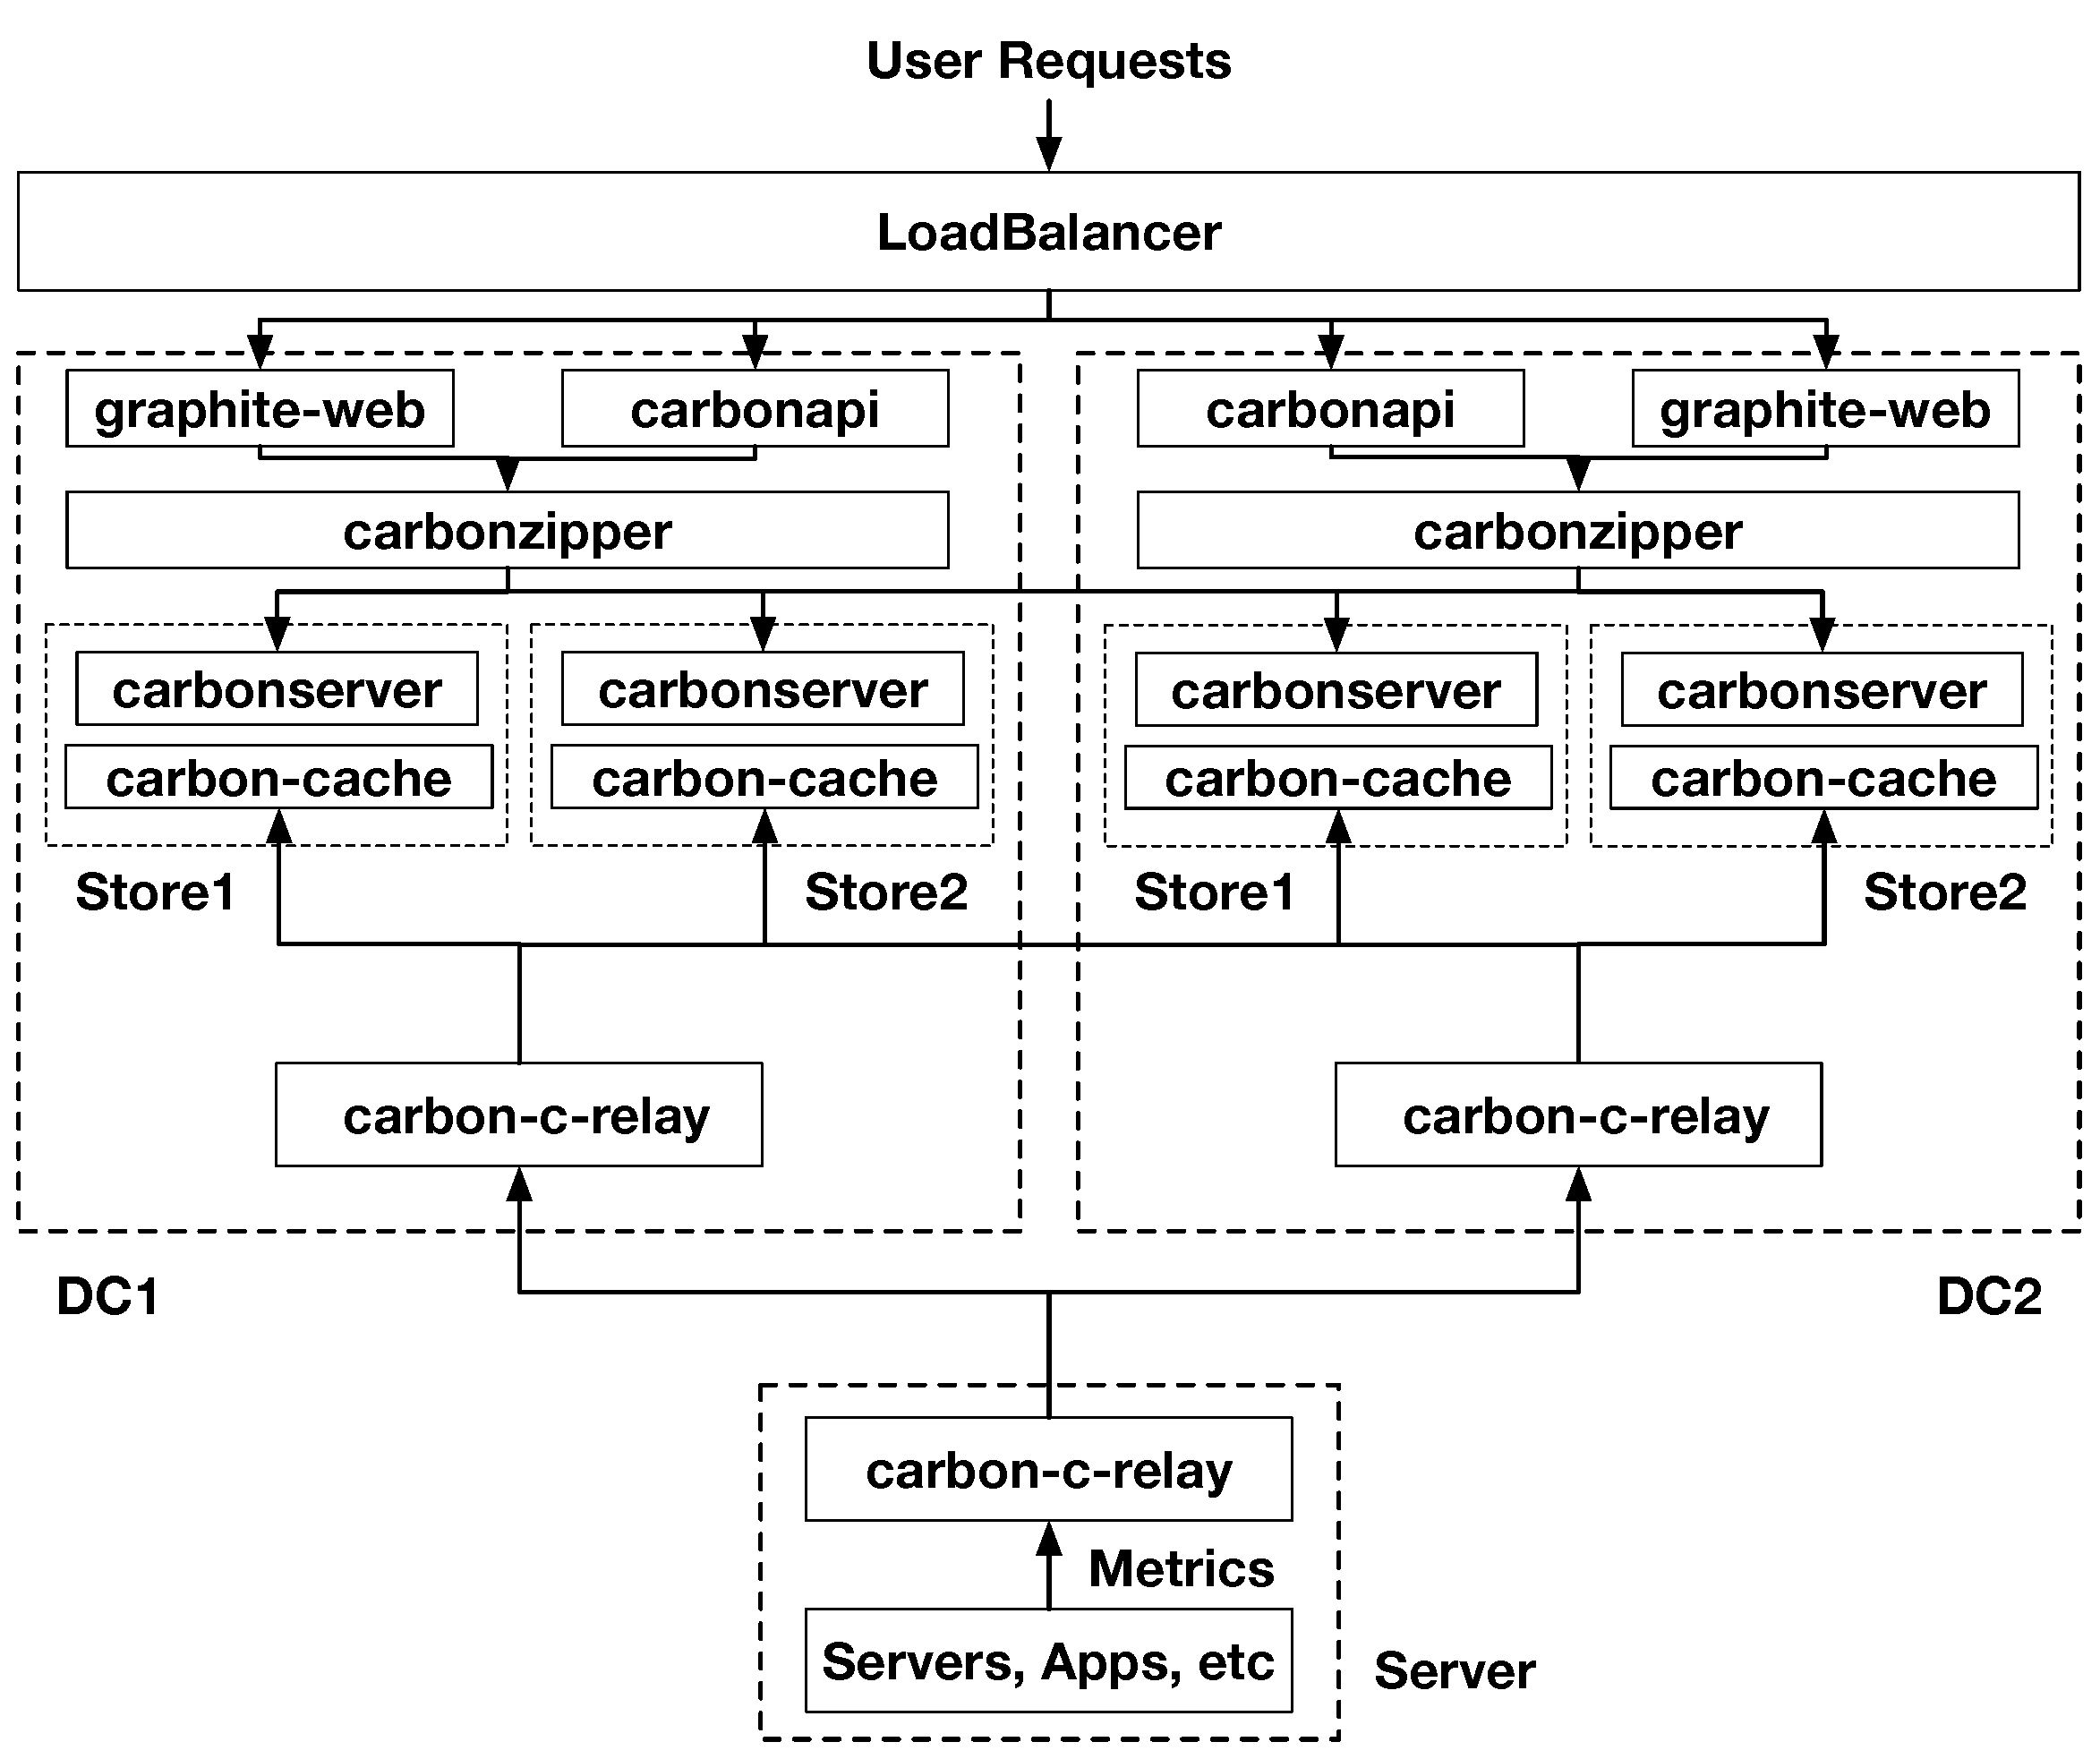
\includegraphics[width=0.8\columnwidth]{graphite-current}
%		\end{center}
%	\end{figure}
	\Large{
	\begin{itemize}
		\item \bs{32} Frontend Servers
		\item \bs{400} RPS on Frontend
		\item \bs{40k} Metric Requests per~second
		\item \bs{11 Gbps} traffic on the backend
		\item \bs{200} Store servers in 2 DCs
		\item \bs{2.5M} unique metrics per~second (\bs{10M} hitting stores)
		\item \bs{130 TB} of Metrics in total
		\item Replaced \bs{all} the components
	\end{itemize}
	\vspace{2.5em}
	}
\end{frame}

\begin{frame}
	\frametitle{What's next?}
	\Large{
	\begin{itemize}
		\item Metadata search (in progress)
		\item Find a replacement for Whisper (in progress)
		\item Rethink aggregators
		\item Replace graphite line protocol between components
	\end{itemize}
	}
\end{frame}

\begin{frame}
	\frametitle{Bonus 0: carbonsearch --- WIP tags support in graphite}
	Example: target=sum(virt.v1.*.dc:datacenter1.status:live.role:graphiteStore.text-match:metricsReceived)

	\begin{itemize}
		\item Separate tags stream and storage
		\item No history (yet)
		\item No negative match support (yet)
		\item Only "and" syntax
		\item Just a few months old
	\end{itemize}
\end{frame}

\begin{frame}
	\frametitle{Bonus 1: testing Clickhouse on a single server}
	\begin{figure}[h]
		\begin{center}
			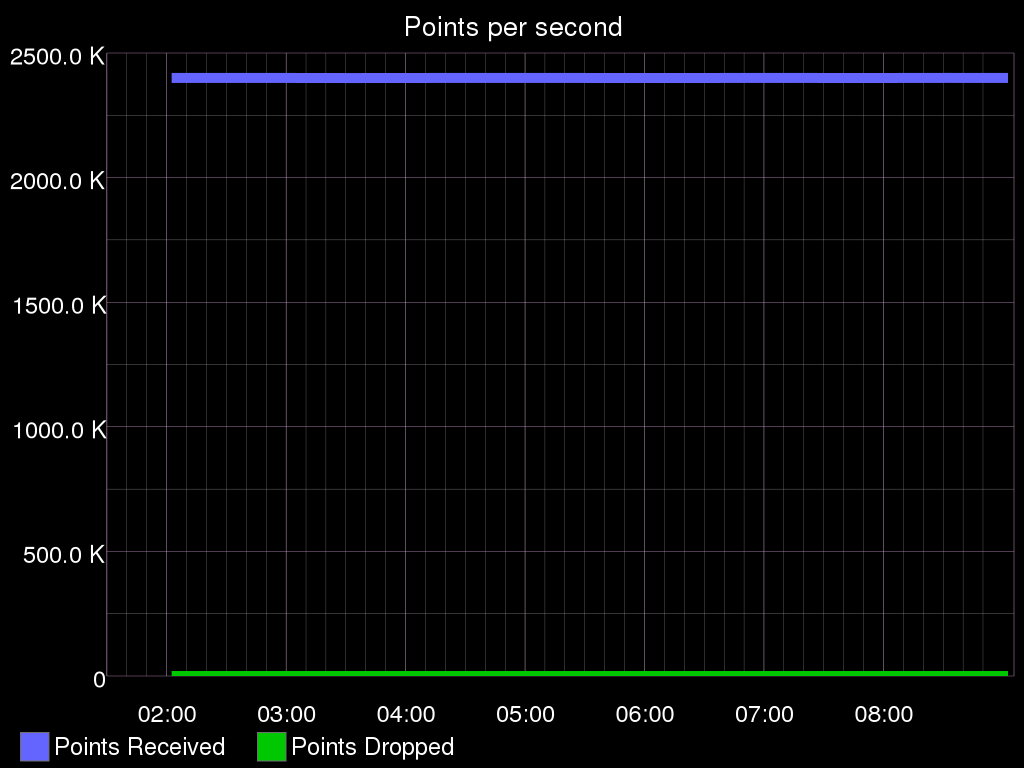
\includegraphics[width=0.8\columnwidth]{clickhouse_experiment_single_server}
		\end{center}
	\end{figure}
\end{frame}


\begin{frame}
	\frametitle{It's all Open Source!}
	\Large{
	\begin{itemize}
		\item carbonzipper --- \href{https://github.com/dgryski/carbonzipper}{github.com/dgryski/carbonzipper}
		\item go-carbon --- \href{https://github.com/lomik/go-carbon}{github.com/lomik/go-carbon}
		\item carbonsearch --- \href{https://github.com/kanatohodets/carbonsearch}{github.com/kanatohodets/carbonsearch}
		\item carbonapi --- \href{https://github.com/dgryski/carbonapi}{github.com/dgryski/carbonapi}
		\item carbon-c-relay --- \href{https://github.com/grobian/carbon-c-relay}{github.com/grobian/carbon-c-relay}
		\item carbonmem --- \href{https://github.com/dgryski/carbonmem}{github.com/dgryski/carbonmem}
		\item replication factor test --- \href{https://github.com/Civil/graphite-rf-test}{github.com/Civil/graphite-rf-test}
	\end{itemize}
	}
\end{frame}

\begin{frame}
\begin{block}{}
        \center\LARGE Questions?

	\center\LARGE \href{mailto:vladimir.smirnov@booking.com}{vladimir.smirnov@booking.com}
\end{block}
\end{frame}


\begin{frame}
\frametitle{What's next?}
\begin{block}{}
        \center{
		\LARGE{Thanks!}

	%	\vspace{2em}
	%	We are hiring!

	%	\href{https://workingatbooking.com/}{https://workingatbooking.com}
	}
\end{block}
\end{frame}

\end{document}
